\documentclass[11pt,letterpaper]{article}
\usepackage[T1]{fontenc}
\usepackage[utf8]{inputenc}
\usepackage[margin=1in,headheight=15pt]{geometry}
\usepackage{microtype}
\usepackage{amsmath,amsthm,mathtools}
\usepackage{newpxtext,newpxmath}
\usepackage{booktabs,longtable,array}
\usepackage{xcolor}
\usepackage{enumitem}
\usepackage{listings}
\usepackage{fancyhdr}
\usepackage{tikz}
\usetikzlibrary{arrows.meta,positioning}
\usepackage[most]{tcolorbox}
\usepackage{hyperref}
\usepackage[nameinlink,noabbrev]{cleveref}
\definecolor{ink}{HTML}{18374A}
\definecolor{accent}{HTML}{197A7C}
\definecolor{wash}{HTML}{F1F6F7}
\hypersetup{colorlinks=true,linkcolor=ink,citecolor=accent,urlcolor=accent,
 pdftitle={Beyond Halting: A Progress-Modulus Hierarchy for Diophantine Liveness},
 pdfauthor={Research manuscript prepared with ChatGPT},pdfsubject={Computability, Diophantine representation, recurrence, hyperimmune-free degrees}}
\pagestyle{fancy}
\fancyhf{}
\fancyhead[L]{\small\textsc{Beyond Halting}}
\fancyhead[R]{\small Diophantine liveness}
\fancyfoot[C]{\thepage}
\renewcommand{\headrulewidth}{0.3pt}
\setlength{\parskip}{0.35em}
\setlength{\parindent}{1.2em}
\setlist{itemsep=0.3em,topsep=0.4em}
\emergencystretch=2em
\newtheorem{theorem}{Theorem}[section]
\newtheorem{lemma}[theorem]{Lemma}
\newtheorem{proposition}[theorem]{Proposition}
\newtheorem{corollary}[theorem]{Corollary}
\theoremstyle{definition}
\newtheorem{definition}[theorem]{Definition}
\newtheorem{example}[theorem]{Example}
\newtheorem{question}[theorem]{Research question}
\theoremstyle{remark}
\newtheorem{remark}[theorem]{Remark}
\newcommand{\N}{\mathbb N}
\newcommand{\Z}{\mathbb Z}
\newcommand{\Q}{\mathbb Q}
\newcommand{\B}{\{0,1\}}
\newcommand{\Cantor}{\B^{\N}}
\newcommand{\sig}[1]{\Sigma^{0}_{#1}}
\newcommand{\ppi}[1]{\Pi^{0}_{#1}}
\newcommand{\an}{\Sigma^{1}_{1}}
\newcommand{\Buchi}{\mathsf{B}}
\newcommand{\Clock}{\mathsf{CD}}
\newcommand{\Gap}{\mathsf{BG}}
\newcommand{\Fixed}{\mathsf{D}}
\newcommand{\Reach}{\mathsf{Reach}}
\newcommand{\Comp}{\mathsf{Comp}}
\newcommand{\Rat}{\mathsf{Rat}}
\newcommand{\Fin}{\mathsf{Fin}}
\newcommand{\HIF}{\mathsf{HIF}}
\newcommand{\pref}{\mathord{\upharpoonright}}
\newcommand{\treepath}[1]{[#1]}
\newcommand{\code}[1]{\texttt{#1}}
\newcommand{\ind}{\mathbf 1}
\newcommand{\cE}{\mathcal E}
\newcommand{\cK}{\mathcal K}
\newcommand{\cB}{\mathcal B}
\newcommand{\cC}{\mathcal C}
\newcommand{\cT}{\mathcal T}
\newcommand{\rules}{\mathcal R}
\newcommand{\zeros}{\operatorname{Zero}_{\N}}
\newcommand{\dom}{\operatorname{dom}}
\newcommand{\graph}{\operatorname{graph}}
\newcommand{\cyl}[1]{\langle #1\rangle}
\lstset{basicstyle=\small\ttfamily,breaklines=true,columns=fullflexible,
 frame=single,rulecolor=\color{ink!25},backgroundcolor=\color{wash},
 showstringspaces=false,tabsize=4}
\newtcolorbox{resultbox}{colback=wash,colframe=accent,boxrule=0.6pt,
 arc=1mm,left=3mm,right=3mm,top=2mm,bottom=2mm,breakable}

\begin{document}
\begin{titlepage}
\vspace*{0.6in}
{\large\color{accent}\textsc{Research article and exact certificate implementation}}\par
\vspace{0.35in}
{\Huge\bfseries\color{ink} Beyond Halting}\par
\vspace{0.17in}
{\LARGE A Progress-Modulus Hierarchy\par for Diophantine Liveness}\par
\vspace{0.25in}
{\large Effective compactness, scheduler degrees, and\par rational piecewise-affine computation}\par
\vspace{0.4in}
{\large Prepared for the ProveIt research program}\par
{\normalsize September 30, 2026}\par
\vspace{0.35in}
\begin{resultbox}
\textbf{Central equivalence.} For a computable binary-controlled system,
there is a recurrent run with a computable progress deadline if and only if
its accepting schedules contain a nonempty effectively closed subset,
if and only if it has an accepting scheduler of hyperimmune-free degree.

\textbf{Sharp classification.} Finite reachability, a fixed recurrence
deadline, some bounded-gap guarantee, some computable deadline, and
unrestricted existential recurrence have respective worst-case complexities
\[
 \sig1,\qquad \ppi1,\qquad \sig2,\qquad \sig3,\qquad \an.
\]
All five are realized by one fixed two-stack system and its exact rational
piecewise-affine realization.
\end{resultbox}
\vfill
\small
\textbf{Status.} This is a research manuscript with detailed mathematical proofs
and a tested finite-horizon compiler, not a claim of a new proof of MRDP,
a solution of the finite-fold conjecture, or established publication priority.
The basis theorems and classical recurrence hardness are explicitly attributed.
The integrated progress-clock formulation, exact compiler, and applications
are developed here. No new Lean formalization is included or claimed.
\end{titlepage}

\begin{abstract}
The Matiyasevich--Robinson--Davis--Putnam theorem represents finite successful
computations by existential polynomial equations. It does not represent every
property of a universal computational substrate: the temporal predicate and
its quantifiers matter. We analyze existential recurrent reachability in
computable, finitely branching systems through \emph{progress deadlines}.
A shared deadline converts recurrence into an effectively closed condition;
checking each finite horizon independently without retaining earlier deadlines
does not. We prove a three-way equivalence between a computable deadline,
a nonempty effectively closed family of accepting schedules, and an accepting
schedule of hyperimmune-free Turing degree. We give full upper-bound and
hardness constructions for the resulting arithmetical/analytical hierarchy,
separate computable clocks from computable schedulers, and construct a system
with recurrent runs but no computable deadline. More generally, every c.e.
Turing degree is realized as the exact minimum oracle degree needed to
compute a successful deadline.

An explicit two-stack compiler produces a nonnegative quartic polynomial
whose natural zeros correspond bijectively to rule-labelled finite runs
satisfying all prescribed deadlines. With horizon $H$, $R$ rules, $G$ top
guards, $E$ empty guards, and $k$ deadlines, it uses exactly
$H(3+R+G)+k$ variables and $H(4R+E+2G+2)+k$ quadratic residuals.
The same semantics are realized by a fixed guarded rational piecewise-affine
relation on a compact three-dimensional cube. A fourth coordinate internalizes
the scheduler as an initial real parameter, yielding a deterministic map.
We explain the different classifications for rational, computable, and
unrestricted initial parameters, derive fixed-arity polynomial quantifier
normal forms using ProveIt's MRDP interface, and specify concrete subsequent
formalization and research tasks. The accompanying dependency-free Python
implementation includes exact arithmetic tests and an exported sample
certificate.
\end{abstract}

\begingroup
\setlength{\parskip}{0pt}
\small
\tableofcontents
\endgroup
\newpage

\section{The research question and the contribution boundary}\label{sec:intro}

\subsection{What follows from universality, and what does not}
Suppose a computational model has finitely encoded configurations, an
effective finite execution semantics, and a finite event recognized by a
semidecision procedure. Its successful finite executions form a computably
enumerable relation. MRDP \cite{matiyasevich1970} then yields a fixed finite polynomial with natural
witnesses for that relation. This reasoning is independent of whether the
model is a Turing machine, a combinator system, a graph-rewriting machine,
or an exact geometric simulator.

There is an important limit. ``Some computation halts'' and ``some computation
returns to an accepting region infinitely often'' are different predicates.
An infinite execution is not a natural number unless extra restrictions make
it effectively describable, and existential quantification over all schedules
cannot simply be replaced by existential quantification over program indices.
This article asks three precise questions.

\begin{enumerate}[label=\textbf{Q\arabic*.},leftmargin=2.3em]
\item Which finite progress requirements allow the compactness argument that
turns success at every finite horizon into one successful infinite run?
\item Exactly what computational strength is needed for a recurrence schedule
when a computable clock exists?
\item Which of these temporal properties admit ordinary Diophantine
representations, which need alternating number quantifiers, and which need
an infinite witness?
\end{enumerate}

The answers are not merely the observation that every computably enumerable
relation is Diophantine. They identify the semantic obstruction, characterize
its degree-theoretic boundary, and connect it to a concrete polynomial
compiler and an unconventional geometric realization.

\subsection{Repository anchor and what was inspected}
The ProveIt repository contains a natural-number MRDP interface
\code{Diophantine.mrdp}, its converse \code{Diophantine.mrdp\_iff}, and an
adapter to Mathlib's \code{Dioph} predicate. The inspected theorem has the form
\begin{equation}\label{eq:mrdp}
 S\text{ is c.e.}\quad\Longleftrightarrow\quad
 \exists r\ \exists P\in\Z[X,Y_1,\ldots,Y_r]\ 
 \forall n\in\N:\quad n\in S\leftrightarrow\exists\vec y\in\N^r\ P(n,\vec y)=0.
\end{equation}
Both the polynomial and witness dimension are chosen before the input.
The repository's documentation explicitly separates this existence theorem
from numerical degree bounds and from an executable polynomial-extraction
algorithm \cite{proveit-mrdp,proveit-guide}.

For reproducibility, the actual public MRDP source was inspected at commit
\begin{center}
\small\code{b6bf6406a4c49017fedc6fba068b36c634987150}.
\end{center}
The MRDP guide and the Turing-degree project README were also inspected at
revision \code{b998f70c6886e6a00339a6f4a02ed8625324d357}.
These are source inspections, not a fresh build or an independent audit of
every repository theorem. The present proofs use ordinary MRDP as a classical
backend and do not rely on unrelated repository claims. The Turing-degree
README distinguishes its basic Lean theory from deeper Rocq developments and
from the separately conditional coarse-degree library \cite{proveit-degrees}.
No conditional coarse-degree theorem is used here.

\subsection{Prior work and the novelty ledger}
Recurrent computations were already used to obtain analytical-hierarchy
hardness in the work of Harel, Pnueli, and Stavi; their recurrence problem is
also explicitly recalled by Esparza and Krasotin \cite{hps,ek2025}.
Thus the $\an$ endpoint below is a classical phenomenon, not a new
undecidability breakthrough. Jockusch and Soare's low and hyperimmune-free
basis theorems are likewise classical \cite{js1972}; domination and its
interaction with effectively closed classes are studied further in
\cite{ng2013}. We use these results with explicit hypotheses.

Finitary acceptance asks for an unknown finite response bound.
Chatterjee and Fijalkow investigate this in an automata-theoretic setting
\cite{cf2011}. Their Borel classifications concern sets of infinite words;
our hierarchy classifies \emph{sets of finite input indices}. These are
not the same hierarchy. Moore's work supplies early dynamical universality
precedent \cite{moore1990}. Our geometric section is an elementary exact
construction for controlled guarded affine maps; it asserts neither
continuity nor noise-robust physical computation.

\begin{center}
\begin{tabular}{@{}p{0.31\linewidth}p{0.62\linewidth}@{}}
\toprule
Result or component & Status in this article\\
\midrule
MRDP; low and HIF basis theorems & Classical ingredients, cited and separated from the new construction.\\
Analytical recurrence hardness & Classical endpoint, with a self-contained reduction supplied.\\
Clock/closed-class/HIF equivalence & Derived here in one operational formulation; no priority claim.\\
The full clock hierarchy & Complete proofs and timing-safe universal realizations supplied here.\\
C.e.-degree clock spectra & Explicit uniform realization of every c.e. degree; proof supplied here.\\
Exact two-stack quartic compiler & Explicit construction, exact counts, conventional proof, finite tested implementation.\\
Geometric and parameter regimes & Constructive consequences with the quantified initial-data domain stated explicitly.\\
Lean certification of these additions & Not performed; an integration plan is given.\\
\bottomrule
\end{tabular}
\end{center}

The substantive outcome is a unified theorem package and an implementable
arithmetization boundary, rather than an unsupported assertion that a
longstanding named conjecture has been settled. Independent mathematical
review and a wider priority search remain appropriate.

\section{Operational semantics and progress clocks}\label{sec:model}

\subsection{A fixed binary-controlled effective system}
\begin{definition}\label{def:system}
A \emph{computable binary-controlled system} consists of natural-number-coded
configurations $c$, a total computable transition function
$\delta(c,b)$ for $b\in\B$, a computable initial configuration $i(e)$ for
finite input $e\in\N$, and a decidable accepting predicate $A(c)$.
A schedule $f\in\Cantor$ determines
\[
 c_0=i(e),\qquad c_{t+1}=\delta(c_t,f(t)).
\]
Halting, disabled actions, or invalid configurations can be completed by an
absorbing rejecting sink. A schedule is an arbitrary infinite bit sequence,
not necessarily computable.
\end{definition}

The transition computation is total; therefore the finite run determined
by a finite bit string can be computed completely. Deterministic steps may
ignore their action bit. More general effective finite branching can be
encoded by finite action alphabets, but the binary formulation makes the
compactness and degree arguments transparent. For a rule-based compiler,
we retain the rule label as part of the finite trace.

We count accepting visits at times $1,2,\ldots$, excluding the initial time:
\begin{equation}\label{eq:count}
 N_{e,f}(t)=\sum_{u=1}^{t}\ind_{A(c_u)},\qquad
 \tau_{e,f}(k)=\min\{t:N_{e,f}(t)\ge k\}.
\end{equation}
The second expression is defined only when the $k$th visit occurs. We often
suppress $e$ in the notation. The set of accepting schedules is
\begin{equation}\label{eq:buchi-class}
 \cB_e=\{f:\forall k\ge1\ \exists t\ N_{e,f}(t)\ge k\}.
\end{equation}
Thus acceptance is the B\"uchi condition of infinitely many visits.

\begin{definition}\label{def:deadline}
A \emph{deadline} is a strictly increasing function
$d:\N_{>0}\to\N_{>0}$. In particular $d(k)\ge k$.
A schedule meets $d$ when $N_{e,f}(d(k))\ge k$ for every $k\ge1$.
Write
\[
 \cK_{e,d}=\{f:\forall k\ge1\ N_{e,f}(d(k))\ge k\}.
\]
For a finite deadline vector $\vec d=(d(1),\ldots,d(k))$, let
\begin{equation}\label{eq:finite-feasibility}
 \Fin(e,\vec d)\quad\Longleftrightarrow\quad
 \exists\sigma\in\B^{d(k)}\ \forall j\in\{1,\ldots,k\}:\quad
 N_{e,\sigma}(d(j))\ge j.
\end{equation}
The empty vector is feasible. Every earlier deadline is retained.
\end{definition}

For a finite explicit vector, $\Fin$ is decidable: enumerate its finitely
many binary schedules and compute their finite runs. The procedure can be
very expensive, but the hierarchy requires decidability, not an efficient
bound. When $d$ is computable, $(e,k)\mapsto\Fin(e,d\pref k)$ is decidable.

\subsection{Four recurrence predicates and one finite predicate}
For a fixed computable deadline $d$, define
\begin{align}
 \Fixed_d(e)&\iff\cK_{e,d}\ne\varnothing,\label{eq:D}\\
 \Gap(e)&\iff\exists f\ \exists b\ge1\ \forall t\ge0:
       N_{e,f}(t+b)-N_{e,f}(t)\ge1,\label{eq:BG}\\
 \Clock(e)&\iff\exists\text{ a total computable deadline }d:
       \cK_{e,d}\ne\varnothing,\label{eq:CD}\\
 \Buchi(e)&\iff\cB_e\ne\varnothing,\label{eq:B}\\
 \Reach(e)&\iff\exists f\ \exists t\ge1:\ A(c_t).\label{eq:reach}
\end{align}
The gap condition includes the initial delay: the first visit occurs by $b$,
and successive visits are at most $b$ steps apart. Requiring a bound only
after some finite prefix gives the same \emph{existence} predicate, because
a finite prefix and finitely many initial gaps can be absorbed into a larger
bound. However, a linear bound $\tau_f(k)\le bk$ is not the same as a bound
on every individual gap. We never use those two notions interchangeably.

There are immediate inclusions
\begin{equation}\label{eq:inclusions}
 \Fixed_{\mathrm{id}}\ \subseteq\ \Gap\ \subseteq\ \Clock\ \subseteq\ \Buchi,
 \qquad\text{where }\mathrm{id}(k)=k.
\end{equation}
The second inclusion follows by taking $d(k)=bk$.

\section{A shared deadline restores compactness}\label{sec:compact}

\begin{theorem}[Coherent deadline compactification]\label{thm:compact}
For every system, input $e$, and deadline $d$, computable or not,
\begin{equation}\label{eq:compact-equivalence}
 \cK_{e,d}\ne\varnothing
 \quad\Longleftrightarrow\quad
 \forall k\ge1\ \Fin(e,d\pref k).
\end{equation}
When $d$ is computable, $\cK_{e,d}$ is an effectively closed subset of Cantor
space, given uniformly by a computable binary tree.
\end{theorem}
\begin{proof}
For each $j$, the condition $N_{e,f}(d(j))\ge j$ depends only on the first
$d(j)$ bits of $f$. Its solution set $C_j$ is therefore clopen. Feasibility
of the first $k$ deadlines says that
$C_1\cap\cdots\cap C_k$ is nonempty. These intersections are nested compact
sets. Compactness of Cantor space gives a point in their intersection,
which is exactly $\cK_{e,d}$. The reverse implication follows by truncation.

For effectiveness, put a finite string $\sigma$ into $T_{e,d}$ precisely
when it satisfies every deadline $d(j)\le|\sigma|$ that is already due.
Because $d$ is increasing, compute its values until the first one exceeds
$|\sigma|$, then check the finite list of requirements. This is a total
decision procedure, and the tree is prefix closed. Its infinite paths are
exactly $\cK_{e,d}$. The assertion also follows directly from K\"onig's
lemma applied to this finitely branching tree.
\end{proof}

\begin{example}[The incoherent-prefix trap]\label{ex:burst}
Consider a machine that first chooses a natural number $n$ in unary:
$n$ continue steps followed by one stop step. It then emits exactly $n$
accepting pulses, one per step, and enters a rejecting sink. The path that
continues forever emits no pulses. Every run has only finitely many
accepting visits.

Nevertheless, for each $k\ge1$, choosing $n=k$ gives $k$ visits by time
$2k+1$. Hence
\begin{equation}\label{eq:wrong}
 \forall k\ \exists\sigma\in\B^{2k+1}:\quad N_{e,\sigma}(2k+1)\ge k
\end{equation}
is true, while $\Buchi(e)$ is false. With $d(j)=2j+1$, meeting the first
deadline forces $n=1$: the first pulse is at $n+2$, and $n=0$ has no pulse.
That choice cannot meet the second deadline. In particular,
$\Fin(e,(3,5))$ is false.
\end{example}

This example locates the exact error in an attractive but invalid proof:
one cannot interchange the finite witnesses for different requirements
without checking that they belong to a nested family. B\"uchi acceptance
is generally an effective $G_\delta$ condition,
\[
 \cB_e=\bigcap_{k\ge1}\ \bigcup_{t\ge1}
       \{f:N_{e,f}(t)\ge k\},
\]
not a closed condition. A chosen clock replaces each open union by one
finite-prefix requirement.

\begin{proposition}[Closed subsets yield computable clocks]\label{prop:closed-clock}
If $P$ is a nonempty effectively closed subset of $\cB_e$, then there is a
computable deadline $d$ with $P\subseteq\cK_{e,d}$.
\end{proposition}
\begin{proof}
Write $P=[T]$ for a computable binary tree. For a fixed $k$, search for a
level $n$ such that every node $\sigma\in T\cap\B^n$ has
$N_{e,\sigma}(n)\ge k$. Each level test is decidable. If the search never
succeeded, the nodes of $T$ with fewer than $k$ accepting visits would form
an infinite finitely branching subtree. K\"onig's lemma would provide a
path in $P$ with fewer than $k$ visits, contradicting $P\subseteq\cB_e$.
Thus the search terminates. Starting the search above $d(k-1)$ makes the
result strictly increasing, with $d(0)=0$. The finite program implementing
this search computes a deadline valid for every path in $P$.
\end{proof}

The algorithm in this proof uses the promise $\varnothing\ne P\subseteq\cB_e$.
It is not a decision procedure for that promise. This distinction matters
when a proposed compiler tries to synthesize a clock from an unverified
invariant.

\section{Scheduler degrees: an exact characterization}\label{sec:degrees}

\subsection{Hyperimmune-free degrees and a basis argument}
\begin{definition}
A schedule $f$ has \emph{hyperimmune-free degree} when every total function
$g:\N\to\N$ with $g\le_T f$ is bounded by some total computable function.
Using eventual domination instead of pointwise domination gives the same
notion: finitely many exceptional values can be incorporated as constants
in a computable bound. A schedule is \emph{low} when $f'\le_T\varnothing'$.
\end{definition}

The hyperimmune-free basis theorem says that every nonempty effectively
closed subset of Cantor space contains a member of hyperimmune-free degree
\cite{js1972,ng2013}. We record its compactness mechanism because it is
precisely what is needed for clocks.

\begin{lemma}[Classical HIF basis theorem]\label{lem:hifbasis}
Every nonempty effectively closed $P\subseteq\Cantor$ contains an HIF member.
\end{lemma}
\begin{proof}
Construct a nested sequence of nonempty effectively closed classes
$P=P_0\supseteq P_1\supseteq\cdots$, handling the $e$th oracle functional
$\Phi_e$ at stage $e$. If for some $n$ the class
\[
 P_e\cap\{f:\Phi_e^f(n)\uparrow\}
\]
is nonempty, choose such an $n$ and use this class as $P_{e+1}$. It is
effectively closed: nonconvergence is a closed finite-computation condition.
If no such $n$ exists, then $\Phi_e^f(n)$ converges for every $f\in P_e$ and
every $n$.

In the latter case fix a computable tree for $P_e$. For each input $n$, search
for a level $l$ at which every tree node of length $l$ gives a convergent
computation of $\Phi_e(n)$ within $l$ steps, using only the supplied $l$
oracle bits. Such a level exists; otherwise the nonconvergent finite
computations form an infinite subtree and yield a path on which the
functional diverges. The maximum of the finitely many outputs at the
successful level is a computable bound $g_e(n)$. Set $P_{e+1}=P_e$.

Compactness gives $f\in\bigcap_e P_e$. If $\Phi_e^f$ is total, the divergent
restriction could not have been chosen at stage $e$, so $g_e$ bounds it.
Therefore $f$ has HIF degree. The stage choices need not be effective; each
chosen finite tree index is a fixed constant in the corresponding program
for $g_e$. This is an existence proof, not an algorithm selecting an HIF
path from a tree index.
\end{proof}

\subsection{The main equivalence}
\begin{theorem}[Clock--closed-class--degree equivalence]\label{thm:core}
For every input $e$ to a computable binary-controlled system, the following
are equivalent:
\begin{enumerate}[label=\textnormal{(\roman*)}]
\item $\Clock(e)$: some accepting schedule meets a computable deadline;
\item $\cB_e$ contains a nonempty effectively closed subset of Cantor space;
\item $\cB_e$ contains a schedule of hyperimmune-free Turing degree.
\end{enumerate}
Moreover, whenever these conditions hold, $\cB_e$ contains a low schedule.
The low schedule and the HIF schedule are not asserted to be the same.
\end{theorem}
\begin{proof}
For (i)$\Rightarrow$(ii), use the nonempty effectively closed set
$\cK_{e,d}$ from \cref{thm:compact}. The converse is
\cref{prop:closed-clock}. For (ii)$\Rightarrow$(iii), apply the HIF basis
theorem to the closed subclass.

For (iii)$\Rightarrow$(i), let $f\in\cB_e$ be HIF. Given oracle $f$, simulate
the run until the $k$th accepting visit. Because $f$ is accepting, this
algorithm computes the total function $k\mapsto\tau_{e,f}(k)$.
There is a computable bound $h$ for it. The function
\begin{equation}\label{eq:strictify}
 d(k)=k+\max_{1\le j\le k}h(j)
\end{equation}
is computable and strictly increasing, and bounds $\tau_{e,f}(k)$.
Finally, the classical low basis theorem of Jockusch and Soare applied
to $\cK_{e,d}$ supplies a low accepting schedule \cite{js1972}.
\end{proof}

This theorem distinguishes two kinds of information. A computable clock
bounds how late progress may occur; it need not tell us which compatible
branch to choose. Conversely, an HIF schedule may contain noncomputable
information, but cannot use that information to produce a progress-time
function escaping every computable upper bound.

\begin{corollary}[Oracle-relative form]\label{cor:relative}
Let $Z$ be any oracle, and allow the transition function, initial coding,
and acceptance predicate to be computable relative to $Z$.
There is a $Z$-computable deadline met by some accepting schedule if and
only if there is an accepting $f$ such that every total
$g\le_T f\oplus Z$ is dominated by a $Z$-computable function.
\end{corollary}
\begin{proof}
Relativize the effective closed-tree construction, the basis argument, and
the computation of $\tau_{e,f}$ in the preceding proof.
\end{proof}

For an ordinary computable system, the set of oracle degrees that can
compute some adequate deadline is upward closed. The relative theorem
characterizes it without confusing a schedule with a program that prints
that schedule. Determining finer properties of this deadline-degree
spectrum is one of the research questions in \cref{sec:questions}.

\section{The sharp progress-modulus hierarchy}\label{sec:hierarchy}

\subsection{Statement and conventions}
Completeness below means computable many-one completeness for sets of natural
input codes. For a fixed system, the unknown is $e$; neither the transition
function nor the accepting region is changed with $e$. We use the standard
arithmetical normal forms $\exists m\forall k R(e,m,k)$ and
$\exists m\forall k\exists s R(e,m,k,s)$, with total decidable $R$.

\begin{theorem}[Progress hierarchy]\label{thm:hierarchy}
Every computable binary-controlled system has the upper bounds in the middle
column of the following table. There is a single fixed universal system for
which every bound is complete, and which can be implemented as a finite
binary-controlled two-stack machine.
\begin{center}
\begin{tabular}{@{}p{0.52\linewidth}cc@{}}
\toprule
Finite-input property & Complexity & Defining pattern\\
\midrule
Some finite accepting visit, $\Reach$ & $\sig1$ & $\exists n$\\
Some run meets a fixed computable $d$, $\Fixed_d$ & $\ppi1$ & $\forall k$\\
Some run has bounded gaps, $\Gap$ & $\sig2$ & $\exists b\forall n$\\
Some run has a computable deadline, $\Clock$ & $\sig3$ & $\exists m\forall k\exists s$\\
Some run is recurrent, $\Buchi$ & $\an$ & $\exists f\forall k\exists t$\\
\bottomrule
\end{tabular}
\end{center}
For the fixed-deadline row, completeness holds for every fixed computable
strictly increasing $d$, including $d(k)=k$.
\end{theorem}

\subsection{Finite reachability and a fixed clock}
For $\Reach$, enumerate finite schedules and simulate them. This semidecides
an accepting visit. To reduce halting, simulate an ordinary program without
accepting and enter an accepting state exactly when it halts. The finite
input encodes the simulated program, so one interpreter handles the entire
reduction.

For $\Fixed_d$, \cref{thm:compact} gives the $\ppi1$ definition
$\forall k\,\Fin(e,d\pref k)$. For hardness, simulate a program while
marking every nonhalting interpreter microstep accepting. If it halts,
enter a rejecting sink. Nonhalting produces one accepting visit at every
time and therefore satisfies every $d(k)\ge k$. Halting produces only
finitely many accepting visits and satisfies no deadline. This reduces
the complement of the halting problem to $\Fixed_d$.

\subsection{An unknown bounded-gap guarantee}
Fix $b\ge1$. A finite schedule of length $n$ is $b$-admissible when every
window $(t,t+b]$ contained in that finite prefix contains an accepting
visit. Checking that a $b$-admissible schedule of length $n$ exists is
decidable. These conditions define a prefix-closed binary tree; K\"onig's
lemma gives
\[
 \exists f\ \forall t\ge0:\ N_f(t+b)-N_f(t)\ge1
 \quad\Longleftrightarrow\quad
 \forall n\ \exists\text{ a $b$-admissible prefix of length }n.
\]
The finite existential search is part of the decidable matrix. Quantifying
$b$ gives a $\sig2$ upper bound.

For hardness, let $S(e)\leftrightarrow\exists m\forall k R(e,m,k)$, with
$R$ decidable. The system first guesses $m$ in unary without accepting.
After the guess ends, it deterministically checks
$R(e,m,0),R(e,m,1),\ldots$. All computation steps during these checks are
accepting. On the first false test it enters the rejecting sink.

If some $m$ works, the finite guessing prefix is followed by an accepting
visit at every step, so some gap bound holds. If no $m$ works, every completed
guess eventually reaches the sink. A schedule that never finishes guessing
has no accepting visits. Thus $\Gap$ holds exactly when $S(e)$ holds.
The acceptance flag during verification is essential: the computation times
of the individual decidable tests need not have a uniform bound.

\subsection{An unknown total computable deadline}
Fix an effective enumeration $(\varphi_m)$ of partial computable functions.
There is a decidable predicate $V(e,m,k,s)$ saying:
\begin{quote}
By computation stage $s$, all values $\varphi_m(1),\ldots,\varphi_m(k)$
have halted, are positive and strictly increasing, and their resulting
finite deadline vector is feasible.
\end{quote}
One may either include the finite feasibility computation in the stage bound
or run its total decision procedure after the bounded simulations; both
define decidable predicates with the same existential closure in $s$.
The condition for $k=0$ can be declared true. Then
\begin{equation}\label{eq:CDsigma3}
 \Clock(e)\quad\Longleftrightarrow\quad
 \exists m\ \forall k\ \exists s\ V(e,m,k,s).
\end{equation}
The same index $m$ must serve every $k$. If the right side holds, it defines
a single total computable deadline, and coherent compactification supplies
a run meeting it. This proves the $\sig3$ upper bound.

For hardness, start with
$S(e)\leftrightarrow\exists m\forall k\exists s R(e,m,k,s)$.
Guess $m$ in unary. For $k=0,1,2,\ldots$, search $s=0,1,2,\ldots$ until
$R(e,m,k,s)$ is true; then emit one accepting pulse and advance to $k+1$.
No search step is accepting. If $m$ satisfies the formula, the run obtained
by using the least successful $s$ at each stage is computable and recurrent.
Its $k$th accepting time is therefore a total computable function; strictify
it if necessary to obtain a deadline. If no $m$ satisfies the formula, every
completed guess eventually stalls on a stage with no witness. Infinite unary
guessing produces no pulses. There is then no recurrent run at all, hence
no computable-deadline run. This proves $\sig3$ hardness.

\subsection{Unrestricted recurrence and recursive trees}
The definition $\exists f\forall k\exists t\,N_f(t)\ge k$ is analytic,
so $\Buchi$ belongs to $\an$. For completeness, we spell out the standard
recursive-tree reduction behind this endpoint; the recurrent-machine
hardness itself is classical \cite{hps,ek2025}.

\begin{lemma}[Analytic tree normal form]\label{lem:analytic-tree}
For every $\an$ set $S\subseteq\N$, there is a uniformly primitive-recursive
family of prefix-closed trees $T_e\subseteq\N^{<\N}$ such that
\[
 e\in S\quad\Longleftrightarrow\quad
 \exists g\in\N^\N\ \forall n:\ g\pref n\in T_e.
\]
\end{lemma}
\begin{proof}[Normal-form argument]
Write an analytic definition as an existential function quantifier followed
by an arithmetic formula. Put the finite number-quantifier part in prenex
form and absorb all existential number choices into additional Skolem
functions, dependent on the preceding universal number variables. Encode
these functions and the original function into one $g$. This gives
$\exists g\forall n\,R(e,g,n)$, where $R$ is a total oracle-computable
Boolean test.

For a finite sequence $\sigma$ of length $l$, run the first $l$ tests for
$l$ steps, answering oracle questions within $\sigma$ and suspending a
test that asks outside it. Reject $\sigma$ exactly when a fully evaluated
test is false. This is a primitive-recursive bounded computation and is
prefix closed. A $g$ satisfying every test has all its prefixes in the
tree. Conversely, along an infinite tree path every particular test obtains
all its finitely many oracle answers and finishes at a sufficiently long
stage, so it cannot be false. This proves the equivalence. Standard coding
of the finitely many function components is effective.
\end{proof}

Given $e$, the recurrent machine maintains a finite sequence $\sigma$.
It guesses the next natural $n$ by unary binary choices, appends $n$, checks
$\sigma^\frown n\in T_e$, and emits one pulse exactly when the check
succeeds. A failed check leads to the rejecting sink. The tree check is
always a terminating finite computation. An infinite branch gives an
accepting schedule. Conversely, an accepting schedule must complete
infinitely many guesses and successful checks, so its guessed values form
an infinite branch. Remaining forever inside one unfinished unary guess
cannot create recurrence. This is the reduction.

\subsection{Why one fixed two-stack machine suffices}\label{sec:universal}
The reductions above describe a finite menu of interpreters with input
parameters: a halting simulator, an always-accepting safety simulator,
a unary-witness verifier, a pulse-on-success searcher, and a recursive-tree
checker. A single machine can include these modes in its finite control and
read a mode-tagged program from its initial finite storage.

A two-stack machine simulates an ordinary tape by storing the finite tape
on the two sides of the head, keeping the scanned symbol in finite control.
A fixed binary block code represents the finitely many tape symbols using
stack symbols $1$ and $3$. Reading or modifying a symbol requires finitely
many top tests, pops, and pushes; the fixed universal interpreter has only
finitely many such instruction types. External binary choices are read only
at the intended guessing steps and ignored elsewhere. Rejecting halts are
completed by a sink. This gives one finite rule table with effective finite
input encoding. No minimum rule count or explicit small universal table is
claimed.

The accepting flag is part of the finite control. In the $\ppi1$ and $\sig2$
safety modes it is set during every verification microstep. In the search
and tree modes it is set for exactly one microstep per successful stage.
These choices eliminate hidden assumptions about interpreter overhead.
The natural-number arguments of all normal forms are parameters to the
fixed interpreter, not infinitely many new control states.

The strictness of the arithmetical hierarchy and the existence of
nonarithmetical analytic sets imply that the inclusions in
\cref{eq:inclusions} are strict for such a universal system. We next give
concrete separations that explain their computational meaning.

\section{Explicit separations and exact deadline-degree spectra}\label{sec:examples}

\subsection{A computable clock need not compute a scheduler}
Fix an effective enumeration $(\varphi_e)$ of partial computable
natural-number functions. Define a binary tree $T_{\mathrm{DNR}}$ by
\begin{equation}\label{eq:dnr-tree}
 \sigma\in T_{\mathrm{DNR}},\quad |\sigma|=n
 \quad\Longleftrightarrow\quad
 \forall e<n:\quad
 \bigl[\varphi_e(e)\text{ halts within }n\text{ steps with }b\in\B\bigr]
 \Rightarrow \sigma(e)\ne b.
\end{equation}
Membership is decidable by bounded simulation, and the tree is prefix closed.
An infinite path exists: at each coordinate choose the opposite bit if the
diagonal computation eventually outputs a bit, and choose arbitrarily if it
does not. But no computable path exists. A total computable binary path
would equal $\varphi_j$ for some $j$, so at coordinate $j$ it would eventually
violate its own diagonal requirement.

A verifier requests one new bit at each stage, checks the resulting prefix
against \cref{eq:dnr-tree}, and emits a pulse after success. Every finite
verification terminates. For each fixed stage $k$, its worst-case computation
time over the finitely many possible bit prefixes is computably bounded:
enumerate those prefixes and run the terminating bounded checks. Adding
these bounds gives a computable deadline shared by all genuine infinite
paths. A computable accepting schedule would compute a path by recording
the bits requested at successive stages, which is impossible.

\begin{proposition}[The clock/controller distinction is strict]\label{prop:noncomputable-scheduler}
There is a computable binary-controlled system with $\Clock(e)$ true and
with no computable accepting schedule. In fact, there is such a system with
$\Fixed_{\mathrm{id}}(e)$ true.
\end{proposition}
\begin{proof}
The pulse verifier proves the first assertion. For the stronger assertion,
mark every working microstep of the same verifier accepting, instead of
marking only successful stage completions. A failed check enters the
rejecting sink. Because every finite check terminates and exactly one bit
is requested per stage, an infinite nonsink computation determines an
infinite path of the tree. Therefore the schedules meeting $d(k)=k$ are
exactly the schedules that never fail a check. Such schedules exist, but a
computable one would compute an impossible computable DNR path.
\end{proof}

This example also explains why the compactness and basis arguments cannot
be silently turned into effective selection algorithms. It does not conflict
with the existence of low and HIF paths: those paths need not be computable,
and the two basis applications select potentially different paths.

\subsection{A recurrent computation that requires a halting oracle}
List ordinary programs $M_0,M_1,\ldots$ and let
\[
 B(i)=\max\bigl(\{0\}\cup
      \{\text{halting time of }M_j\text{ on blank input}:j\le i\}
      \bigr).
\]
For a sequence $\sigma$ of length $n$, require that whenever a program
$M_j$ with $j\le i<n$ has halted within $n$ steps, its halting time is at most
$\sigma(i)$. This is a primitive-recursive, prefix-closed tree, and its
infinite paths are exactly the functions $g$ satisfying $g(i)\ge B(i)$ for
all $i$.

Run the unary-guess tree verifier of \cref{sec:hierarchy}. Choosing $g=B$
gives an accepting run. Every accepting schedule computes a path $g$, and
such a path decides halting: to test $M_i$, simulate it for $g(i)$ steps.
Also, guessing $g(i)$ in unary costs at least $g(i)$ microsteps before the
$(i+1)$st accepting pulse. Hence any successful deadline satisfies
\[
 B(i)\le g(i)\le\tau_f(i+1)\le d(i+1).
\]
A computable deadline would decide the halting problem. No such deadline
exists, although an accepting run does. The next theorem gives the exact
generalization to every c.e. degree.

\subsection{Realizing arbitrary c.e. deadline lower bounds}
Let $(A_s)_{s\in\N}$ be a computable increasing sequence of finite sets
with union $A$, so $A$ is computably enumerable. Fix a stage convention and
write $t_A(x)$ for the first stage at which $x$ enters $A$, when it does.
Define its finite-initial-segment enumeration modulus
\begin{equation}\label{eq:enum-modulus}
 b_A(i)=\max\bigl(\{0\}\cup\{t_A(x):x\le i,\ x\in A\}\bigr).
\end{equation}
The function $b_A$ is computable from $A$: ask which of $0,\ldots,i$ enter,
then enumerate until all those positive answers have appeared. Conversely,
any pointwise upper bound $h$ for $b_A$ computes $A$, since
\begin{equation}\label{eq:decide-c.e.}
 x\in A\quad\Longleftrightarrow\quad x\in A_{h(x)}.
\end{equation}

\begin{definition}
For a system input $e$, its \emph{deadline oracle spectrum} is
\[
 \operatorname{Spec}_{\mathrm{clk}}(e)=
 \{\deg_T(Z):\text{ some $Z$-computable deadline is met by a run on }e\}.
\]
This records oracle capabilities, not the degrees of every individual
schedule. In particular, the accepting schedule need not be computable
from the oracle that computes the deadline.
\end{definition}

\begin{theorem}[Exact realization of every c.e. degree]\label{thm:ce-spectrum}
Uniformly from an index for a c.e. set $A$, one can construct an input $e_A$
to a fixed binary-controlled two-stack system such that
\begin{equation}\label{eq:spectrum}
 \operatorname{Spec}_{\mathrm{clk}}(e_A)
   =\{\mathbf z:\deg_T(A)\le\mathbf z\}.
\end{equation}
Every accepting scheduler computes $A$, and an $A$-computable accepting
scheduler exists. Consequently its least accepting-scheduler degree and
its least deadline-oracle degree are both $\deg_T(A)$.
The same result holds for the fixed rational guarded affine realization
constructed in \cref{sec:geometry}.
\end{theorem}
\begin{proof}
Define a tree $T_A$ on natural sequences. A sequence $\sigma$ of length $n$
is in $T_A$ when
\begin{equation}\label{eq:c.e.-tree}
 \forall i<n\ \forall x\le i:\quad
 x\in A_n\ \Rightarrow\ t_A(x)\le\sigma(i).
\end{equation}
All entry stages needed in this formula can be computed by looking only at
the finite enumeration through stage $n$. Thus the tree is uniformly
computable, and under a bounded universal-enumeration convention it is
primitive recursive. It is prefix closed because shortening a sequence
only removes coordinates and reduces the enumeration stage inspected.
Its infinite paths are exactly the $g$ with $g(i)\ge b_A(i)$ for all $i$.
Indeed, an eventual enumeration at stage $s$ is enforced by all sufficiently
long prefixes $n\ge\max(s,i+1)$, and the reverse implication is immediate.

The fixed tree-verification interpreter takes the enumeration index as
part of its finite input. It guesses each $g(i)$ in unary, checks the next
prefix, and pulses on success. From an accepting schedule $f$, simulate the
run and recover each completed unary value; this computes $g$ from $f$.
Equation \eqref{eq:decide-c.e.} then computes $A$, so $A\le_T f$.
Taking $g=b_A$, which is $A$-computable, and using a default bit at every
ignored action step gives an $A$-computable accepting schedule.

Now suppose a $Z$-computable deadline $d$ is met by some accepting schedule,
not assumed $Z$-computable. Unary guessing gives
\[
 b_A(i)\le g(i)\le\tau_f(i+1)\le d(i+1).
\]
The $Z$-computable function $i\mapsto d(i+1)$ therefore decides $A$ by
\cref{eq:decide-c.e.}. Hence $A\le_T Z$.
Conversely, if $A\le_T Z$, use the $A$-computable schedule just constructed
and simulate its successive accepting times with oracle $Z$. They form a
$Z$-computable deadline. This proves \cref{eq:spectrum}, as well as the
least-degree assertions. The geometric realization is step-exact, so the
same inequalities and clocks are preserved there.
\end{proof}

This is a useful concrete form of the clock obstruction: it can have any
c.e. degree, not just the full halting degree. It also strengthens a purely
negative statement. The construction identifies exactly which oracles are
sufficient, and it supplies a matching least-degree accepting schedule.
The ingredients are enumeration moduli and recursive trees; the theorem
packages them as a uniform liveness and exact-substrate realization.

\begin{corollary}\label{cor:halting-spectrum}
There is an input with recurrent runs but no computable deadline, whose
deadline oracle spectrum is exactly the upper cone of $\mathbf0'$.
There is a $\mathbf0'$-computable accepting schedule and a
$\mathbf0'$-computable deadline, but every accepting schedule computes
$\mathbf0'$.
\end{corollary}
\begin{proof}
Take $A$ to be the halting set in \cref{thm:ce-spectrum}.
\end{proof}

\subsection{Computable schedules are a different \texorpdfstring{$\sig3$}{Sigma-3} property}
Let $\Comp(e)$ mean that an accepting schedule is computable.
There is a $\sig3$ upper bound: existentially choose a program index,
then require that for every $k$ some finite simulation produces enough
schedule bits for $k$ accepting visits, while verifying totality on the
first $k$ inputs. A single larger finite stage combines these requirements.
The $\sig3$ hardness construction in \cref{sec:hierarchy} already produces
a computable accepting schedule in every positive instance and no accepting
schedule in any negative instance. Thus $\Comp$ is $\sig3$-complete for
the fixed universal system.

Every computable accepting schedule has computable accepting times, so
$\Comp\subseteq\Clock$. The DNR example makes this inclusion strict.
Equal completeness classifications do not identify the underlying
semantics. In particular, existential quantification over program indices
represents $\Comp$, not arbitrary $\Buchi$ acceptance.

\section{The deterministic specialization}\label{sec:deterministic}
If the transition ignores the action bit, an input has a unique computable
run. This removes the source of the analytical jump.

\begin{theorem}[Deterministic boundary]\label{thm:deterministic}
For a computable deterministic system,
\[
 \Clock(e)\quad\Longleftrightarrow\quad\Buchi(e).
\]
The common predicate is $\ppi2$ in general and $\ppi2$-complete for a
suitable fixed deterministic two-stack system. Finite reachability,
fixed-deadline recurrence, and bounded-gap recurrence have sharp bounds
$\sig1$, $\ppi1$, and $\sig2$, respectively.
\end{theorem}
\begin{proof}
A recurrent computable run yields a program computing its $k$th accepting
time by simulation, so it yields a computable deadline. Conversely every
deadline entails recurrence. For the unique run, the condition
$\forall k\exists t\,N_e(t)\ge k$ has a decidable matrix. To obtain
$\ppi2$ hardness, on program index $p$ sequentially simulate
$\varphi_p(0),\varphi_p(1),\ldots$, emitting one pulse after each halt.
The run is recurrent exactly when $\varphi_p$ is total. More generally,
the same construction implements any $\forall k\exists s$ decidable
normal form.

The reachability and fixed-deadline lower bounds in
\cref{sec:hierarchy} are already deterministic. For bounded gaps, the
unique run yields the upper bound $\exists b\forall t$ directly.
For hardness, use the $\sig2$-complete finiteness problem for a c.e. set
$W_p$. Run a standard staged enumerator, marking all ordinary work steps
accepting. At the $j$th distinct enumeration event, insert a nonaccepting
block of at least $j$ microsteps and then resume ordinary work. Each stage
and each inserted block is finite. If $W_p$ is finite, only finitely many
nonaccepting blocks occur, so a gap bound exists. If $W_p$ is infinite,
nonaccepting blocks have unbounded lengths, so no gap bound exists.

For completeness, finiteness of c.e. sets has the required hardness by a
standard moving-candidate construction. Given
$\exists m\forall k R(e,m,k)$, at stage $s$ let $m_s$ be the least
$m\le s$ passing all tests $k\le s$, or let $m_s=s+1$ if there is none.
Enumerate a fresh number whenever $m_s$ changes. If there is a least true
witness $m$, all smaller false candidates are eventually excluded and
$m_s$ stabilizes at $m$. If no witness exists, every finite candidate is
eventually excluded and $m_s$ changes infinitely often. This reduces the
normal form to finiteness. These procedures are modes of one fixed
deterministic interpreter, with accepting flags as above.
\end{proof}

\begin{center}
\begin{tabular}{@{}lcc@{}}
\toprule
Property & Controlled universal system & Deterministic universal system\\
\midrule
Finite reachability & $\sig1$ & $\sig1$\\
Fixed computable deadline & $\ppi1$ & $\ppi1$\\
Some finite gap bound & $\sig2$ & $\sig2$\\
Some computable deadline & $\sig3$ & $\ppi2$\\
Unrestricted recurrence & $\an$ & $\ppi2$\\
\bottomrule
\end{tabular}
\end{center}
Every entry denotes completeness for the corresponding fixed universal
system. Infinite behavior by itself does not force analytic complexity;
existential quantification over arbitrary compatible schedules does.

\section{Exact quartic certificates for two-stack computations}\label{sec:compiler}

\subsection{A canonical natural coding}
A stack word is written top first, $w=d_1\cdots d_l$ with $d_i\in\{1,3\}$.
Use the natural sentinel code
\begin{equation}\label{eq:stackcode}
 \nu(\epsilon)=1,\qquad \nu(dw)=4\nu(w)+d.
\end{equation}
For example,
\[
 \nu(1)=5,\quad \nu(3)=7,\quad\nu(13)=29,\quad\nu(31)=23.
\]
The base-four representation has a leading sentinel $1$; least significant
digits are successive top symbols. This avoids a collision between the
empty word and leading blank symbols. Push and pop are linear equations:
\[
 \text{push }d:\ n'=4n+d,
 \qquad
 \text{pop }d:\ n=4n'+d,\quad n'\ge1.
\]
A top-$d$ guard can be written, with a natural slack $u$, as
\begin{equation}\label{eq:top-slack}
 n=4u+4+d,\qquad\text{so the popped stack is }u+1.
\end{equation}
An empty guard is $n=1$.

\subsection{Rule format and variables}
A finite machine has control labels in $\N$, two stack codes $x,y$, and a
finite labelled rule set $\rules$ of size $R$. A rule $r$ has source
$s_r$, target $t_r$, and one guard/update pair for each stack. Guards are
unrestricted, empty, top-$1$, or top-$3$. Updates are stay, push-$1$,
push-$3$, or pop; a pop requires an explicit top guard. The guards do not
need to be mutually exclusive. Distinct rules remain distinct choices.
Let $G$ be the total number of top guards and $E$ the total number of empty
guards, counted across all rule/stack pairs.

Fix a valid initial configuration $(q_0,x_0,y_0)$ and horizon $H$.
Let $\vec d=(d_1,\ldots,d_k)$ be strictly increasing deadlines with
$1\le d_1<\cdots<d_k\le H$. The initial configuration is substituted as
constants. Introduce the following natural variables:
\begin{center}
\begin{tabular}{@{}p{0.65\linewidth}r@{}}
\toprule
Coordinates & Number\\
\midrule
$q_t,x_t,y_t$, for $1\le t\le H$ & $3H$\\
Rule indicators $e_{t,r}$, for $0\le t<H$, $r\in\rules$ & $HR$\\
A top-guard slack $u_{t,r,a}$ for each top guard on stack $a$ & $HG$\\
Deadline surplus $w_j$, for $1\le j\le k$ & $k$\\
\bottomrule
\end{tabular}
\end{center}
The total is
\begin{equation}\label{eq:Ncount}
 N=H(3+R+G)+k.
\end{equation}
We now give all the polynomial equations; there is no hidden trace-coding
or existential validity predicate.

\subsection{The quadratic residuals}
For each step $t$, impose Booleanity and one-hot selection:
\begin{align}
 e_{t,r}(e_{t,r}-1)&=0 &&(r\in\rules),\label{eq:boolean}\\
 \sum_{r\in\rules}e_{t,r}-1&=0.\label{eq:onehot}
\end{align}
Impose source control and target control:
\begin{align}
 e_{t,r}(q_t-s_r)&=0 &&(r\in\rules),\label{eq:source}\\
 q_{t+1}-\sum_{r\in\rules}t_r e_{t,r}&=0.\label{eq:target}
\end{align}
For an empty guard on a stack value $n_t$, impose
\begin{equation}\label{eq:empty}
 e_{t,r}(n_t-1)=0.
\end{equation}
For a top-$d$ guard with its own slack $u=u_{t,r,a}$, impose
\begin{align}
 e_{t,r}(n_t-4u-4-d)&=0,\label{eq:top}\\
 (1-e_{t,r})u&=0.\label{eq:inactive}
\end{align}
The second equation is not optional: it canonically sets the slack of an
inactive rule to zero. Without it, each inactive top guard would contribute
arbitrary spurious witnesses.

For every rule and every stack, impose one gated update residual, chosen
from
\begin{equation}\label{eq:updates}
 \begin{array}{c|l}
 \text{update}&\text{residual}\\ \hline
 \text{stay}&e_{t,r}(n_{t+1}-n_t)\\
 \text{push }d&e_{t,r}(n_{t+1}-4n_t-d)\\
 \text{pop}&e_{t,r}(n_{t+1}-u_{t,r,a}-1).
 \end{array}
\end{equation}
Let $F$ be the accepting control labels. At the end of step $t$ the
acceptance indicator is
\[
 a_{t+1}=\sum_{r:t_r\in F}e_{t,r}.
\]
It is automatically either zero or one on a solution. For each deadline
$d_j$, impose
\begin{equation}\label{eq:deadline-residual}
 \sum_{t=0}^{d_j-1}\ \sum_{r:t_r\in F}e_{t,r}-j-w_j=0.
\end{equation}
Because $w_j\in\N$, this is exactly the assertion of at least $j$ accepting
visits by that deadline; the surplus is uniquely determined.

All residuals have degree at most two. The step-wise residual counts are
\begin{center}
\begin{tabular}{@{}lr@{}}
\toprule
Constraint family & Residuals per step\\
\midrule
Boolean indicators and one-hot sum & $R+1$\\
Source guards and target equation & $R+1$\\
Empty guards & $E$\\
Top guards and inactive-slack equations & $2G$\\
Two stack updates for each rule & $2R$\\
\bottomrule
\end{tabular}
\end{center}
Thus there are exactly
\begin{equation}\label{eq:Mcount}
 M=H(4R+E+2G+2)+k
\end{equation}
listed residuals, including any residual that simplifies to the zero
polynomial for a special instance. Retaining those listed residuals is the
counting convention implemented by the prototype.

\subsection{The polynomial and the bijection theorem}
Let $L_1,\ldots,L_M$ denote the residuals above, and put
\begin{equation}\label{eq:quartic}
 Q_{\mathcal M,H,\vec d}=\sum_{i=1}^{M}L_i^2.
\end{equation}
Here $\mathcal M$ denotes the machine; when no confusion is possible
we simply write $Q$. It has integer
coefficients and degree at most four, and is nonnegative on every real
assignment.

\begin{theorem}[Exact finite-trace compiler]\label{thm:compiler}
For every finite two-stack machine, canonical initial stacks, horizon $H$,
and deadline vector $\vec d$, the natural zeros of $Q$ are in bijection
with rule-labelled legal runs of length $H$ satisfying all the deadlines.
The certificate has exactly the variable and listed-residual counts in
\cref{eq:Ncount,eq:Mcount}. In particular, a fixed legal rule-labelled run
has exactly one natural witness assignment when it satisfies the deadlines,
and no assignment otherwise.
\end{theorem}
\begin{proof}
Because all $L_i$ take integer values, $Q=0$ is equivalent to the vanishing
of every residual. The Boolean equations force every $e_{t,r}$ to be zero
or one, and the one-hot equation forces exactly one active rule per step.
The source residual for that rule forces $q_t=s_r$, and the target equation
forces $q_{t+1}=t_r$.

Induct on the step number, starting from the stipulated valid stack codes.
For an empty guard of the active rule, \cref{eq:empty} gives $n_t=1$.
For a top guard, \cref{eq:top} gives
$n_t=4(u+1)+d$ with $u+1\ge1$. As $n_t$ is a canonical stack code, its
least significant digit is precisely the tested top symbol, and its
canonical tail has code $u+1$. The appropriate update equation then
produces exactly the stack resulting from stay, push, or pop. Thus the
next stack code is canonical, completing the induction. No independent
regular-language constraints on intermediate stack codes are needed.

The deadline residuals assert the required inequalities because their
surpluses are natural. This constructs a legal deadline-respecting run
from every natural zero.

Conversely, given a legal labelled run, insert its actual configurations,
set the chosen indicator to one and all others to zero, set each active
top slack to the tail code minus one, set every inactive top slack to
zero, and set $w_j$ to the acceptance count by $d_j$ minus $j$. All variables
are natural and all residuals vanish.

Finally, the labelled run fixes all configurations and indicators. Active
top slacks are fixed by the quotient equation, inactive ones by
\cref{eq:inactive}, and deadline slacks by \cref{eq:deadline-residual}.
This proves uniqueness and hence the bijection. The counts follow from
the explicit inventory, and squaring quadratic residuals proves the degree
bound.
\end{proof}

\begin{remark}[The boundary of the uniqueness claim]\label{rem:singlefold}
The dimension grows with $H$ and the number of deadlines. This is a
variable-size finite certificate, not a single fixed-arity single-fold
representation of arbitrary c.e. sets. Replacing all finite traces by a
fixed-arity MRDP polynomial can introduce additional witnesses; uniqueness
is not asserted to survive that replacement. In particular,
\cref{thm:compiler} does not resolve the finite-fold or single-fold
Diophantine representation questions.
\end{remark}

\subsection{Deadline compactness as a quartic schema}
For a fixed computable deadline $d$, set $H=d(k)$ in the compiler, retaining
all $k$ deadlines. For the two-stack system we obtain the exact equivalence
\begin{equation}\label{eq:schema}
 \Fixed_d(e)\quad\Longleftrightarrow\quad
 \forall k\ge1\ \exists\vec z\in\N^{N(k)}:\ Q_{e,k}(\vec z)=0.
\end{equation}
The varying polynomial and dimension are generated effectively from $e,k$.
Equation \eqref{eq:schema} looks syntactically like a $\ppi2$ assertion if
one treats polynomial solvability as a black box. Its actual complexity is
$\ppi1$: the zeros correspond to a finite decidable set of schedules, and
that entire finite search can be carried out directly. Witness magnitude
is not a reason to ignore known operational bounds.

This is another useful distinction. A Diophantine certificate interface can
hide the fact that its particular instances are decidable. Complexity
classification should use the strongest available semantics, not only the
surface quantifier shape of one encoding.

\section{Which simulations preserve a computable clock?}\label{sec:simulation}

A universality theorem can preserve finite halting while distorting temporal
properties. To transfer the preceding results to an unconventional substrate,
we therefore state a stronger, explicitly timed hypothesis.

\begin{definition}
A \emph{computable signal-faithful block simulation} maps each legal finite
source history to a target history, compatibly with prefixes. Each source
step expands to a nonempty, finite, effectively computable block. Every
infinite target execution from an encoded initial state decodes into such
blocks and projects to a source execution; there are no spurious infinite
internal executions. Accepting visits occur precisely at the ends of blocks
whose corresponding source step ends in an accepting state, with one target
visit per source visit. The projection of finite blocks is effective.
\end{definition}

The condition quantifies over all target executions, not merely those
chosen by a favorable simulator. It excludes, for example, an internal
nondeterministic loop that can generate infinitely many fake accepting
signals without simulating any further source step.

\begin{theorem}[Effective clock transfer]\label{thm:transfer}
For effective finitely branching source systems, a computable signal-faithful
block simulation preserves existential recurrence and the existence of a
computable deadline in both directions. It preserves bounded-gap recurrence
in both directions when block lengths have a uniform finite bound.
Without that bound, forward preservation of bounded gaps can fail.
\end{theorem}
\begin{proof}
The one-to-one correspondence of accepting signals proves the recurrence
assertion. For a fixed encoded input $e$ and source length $n$, enumerate
the finitely many legal histories of length at most $n$. Compute all of
their target expansions and let $g_e(n)$ be the maximum expansion length,
including zero for the empty history. This is a total computable,
nondecreasing function; the effective finite-branching hypothesis is used
exactly here.

If a source schedule meets a computable deadline $d$, its $k$th target pulse
occurs no later than $g_e(d(k))$. The strictly increasing computable function
$k+g_e(d(k))$ is therefore a target deadline. Conversely, each source step
uses at least one target step. On any target run with deadline $d$, the
$k$th source pulse occurs after at most $d(k)$ source steps, so the same
$d$ bounds the projected source run.

If each block has length at most $L$, a source gap bound $b$ becomes a
target gap bound $Lb$; the initial delay obeys the same estimate. A target
gap bound is also a source gap bound because blocks are nonempty.
For failure without a uniform upper bound, take a source that pulses every
step and expand its $n$th step into $n$ nonaccepting steps followed by one
pulse. This is a computable signal-faithful simulation, but the target gaps
are unbounded although its progress clock is computable.
\end{proof}

This theorem provides a practical contract for future translations to
rewriting systems, cellular automata, or reaction-style models. It is not
enough to cite their Turing completeness: one must prove finite effective
branching, total expansion of each block, absence of rogue infinite
executions, and the appropriate correspondence of acceptance signals.
A step-exact simulation is especially valuable, since it preserves a
specified deadline without modification.

\section{A compact rational piecewise-affine substrate}\label{sec:geometry}

\subsection{Finite stacks as rational points}
For a top-first finite word $w=d_1\cdots d_l$, set
\begin{equation}\label{eq:rational-stack}
 \rho(w)=\sum_{i=1}^{l}\frac{d_i}{4^i},\qquad\rho(\epsilon)=0.
\end{equation}
Every such point is rational and belongs to $[0,1)$. The stack operations
become rational affine maps:
\begin{align}
 \rho(dw)&=\frac{\rho(w)+d}{4},\label{eq:affine-push}\\
 \rho(w)&=4\rho(dw)-d.\label{eq:affine-pop}
\end{align}
For a valid nonempty stack, the top-$d$ guard is exactly
\begin{equation}\label{eq:affine-top}
 \rho(w)\in[d/4,(d+1)/4),\qquad d\in\{1,3\}.
\end{equation}
The empty stack is characterized by $\rho(w)=0$. Strict upper endpoints
are intentional: no finite valid tail has coordinate $1$.

Choose distinct rational control levels $z_q\in[0,1]$, for example
$q/(s+1)$ for $s$ finite control labels numbered $0,\ldots,s-1$.
A configuration is represented by
\begin{equation}\label{eq:geometric-config}
 (\rho(w_L),\rho(w_R),z_q)\in[0,1]^3.
\end{equation}
Each rule has rational linear guards and an affine update on these three
coordinates. A finite union of these guarded graphs is a finitely branching
piecewise-affine transition relation. For a binary-controlled machine,
there are two guarded piecewise-affine functions $F_0,F_1$, one per action,
whose pieces are disjoint on valid configurations. The finite guard partition can be refined and completed by a rejecting
sink on its unused regions. This does not assert a finite-guard test for
the entire countable set of finite-stack encodings; noncanonical points
inside the chosen affine pieces may follow the same affine formulas.

\begin{theorem}[Step-exact compact geometric realization]\label{thm:geometry}
There is a fixed binary-controlled rational guarded piecewise-affine system
on $[0,1]^3$, a fixed accepting set given by rational control levels, and a
computable family of rational initial points, for which all the completeness
statements in \cref{thm:hierarchy} hold. The c.e.-degree spectrum realizations
of \cref{thm:ce-spectrum} hold as well. For every finite horizon, the natural
quartic certificates of \cref{thm:compiler} certify its encoded trajectories
with exactly the same deadline and witness counts.
\end{theorem}
\begin{proof}
Apply \cref{eq:rational-stack,eq:geometric-config} to the fixed two-stack
system constructed in \cref{sec:universal}. Equations
\eqref{eq:affine-push}--\eqref{eq:affine-top} show, by induction on the run,
that each rule and its affine piece have the same enabledness, resulting
configuration, and accepting label. The initial point is rational and
computable from the finite input, and every reachable encoded point is a
finite-stack point. Thus the simulation preserves every microstep,
acceptance count, and deadline. The hierarchy and the spectrum results
transfer without overhead. The quartic witnesses use $\nu(w)$, not
$\rho(w)$, to represent exactly the same finite words.
\end{proof}

The compactness of the ambient cube does not turn it into a finite-state
system. Stack denominators and numerators in their alternative natural
coding have no uniform bound. Nor is the guarded relation asserted to be
closed or the functions continuous. Rational interval guards and exact
real arithmetic are part of the mathematical semantics. None of these
statements asserts noise tolerance, experimentally realizable infinite
precision, or a physical solution of the halting problem.

\subsection{One deterministic map with the scheduler in the initial point}
The external control stream can instead be encoded in one more real
coordinate. For $f\in\Cantor$, define
\begin{equation}\label{eq:eta}
 \eta(f)=\sum_{t=0}^{\infty}\frac{1+2f(t)}{4^{t+1}},
 \qquad C=\eta(\Cantor)\subseteq[1/3,1].
\end{equation}
This is a Cantor set with disjoint first-digit regions
\[
 f(0)=0:\quad\eta(f)\in[1/3,1/2],
 \qquad
 f(0)=1:\quad\eta(f)\in[5/6,1].
\]
The digit can therefore be read by rational interval guards. With
$S$ the left shift on schedules,
\begin{equation}\label{eq:shift}
 \eta(Sf)=4\eta(f)-1-2f(0).
\end{equation}
Define a deterministic guarded rational piecewise-affine map on $[0,1]^4$
by
\begin{equation}\label{eq:autonomous}
 \mathcal F(X,z)=\bigl(F_b(X),\ 4z-1-2b\bigr)
 \quad\text{on the first-digit region for }b,
\end{equation}
with an arbitrary rejecting completion elsewhere. For a standard encoded
initial point $(X_e,\eta(f))$, its orbit is exactly the controlled run on
schedule $f$, with one bit consumed at every microstep, including steps
where the action is ignored.

The map $\eta$ preserves Turing degree under the usual effective
representation of reals: $f$ computes arbitrarily accurate rational
approximations to $\eta(f)$ by truncation, while the separated digit regions
allow recovery of each bit from increasingly accurate approximations to
the real. Also, $\eta(f)$ is rational exactly when $f$ is eventually
periodic. Indeed, rational base-four expansions are eventually periodic,
and conversely any eventual period yields a rational geometric series.
The endpoint $1$ is represented by the all-$3$ digit stream and causes no
ambiguity within this digit set.

\begin{theorem}[Initial-parameter hierarchy]\label{thm:initial}
For the fixed deterministic map $\mathcal F$ above, with standard finite
input $e$ determining $X_e$, the following classifications are sharp:
\begin{center}
\begin{tabular}{@{}p{0.70\linewidth}c@{}}
\toprule
Question about a recurrent orbit from $(X_e,z)$ & Complexity\\
\midrule
The scheduler coordinate $z\in C\cap\Q$ is specified as finite input & $\ppi2$\\
Some rational scheduler coordinate $z\in C\cap\Q$ works & $\sig3$\\
Some computable scheduler coordinate $z\in C$ works & $\sig3$\\
Some scheduler coordinate admits a computable progress deadline & $\sig3$\\
Some scheduler coordinate of HIF degree works & $\sig3$\\
Some unrestricted scheduler coordinate $z\in C$ works & $\an$\\
\bottomrule
\end{tabular}
\end{center}
The existential computable-parameter condition is strictly stronger than
the existential computable-deadline condition, despite their equal index
complexity.
\end{theorem}
\begin{proof}
A specified rational scheduler coordinate has an effectively computable
orbit, giving the $\ppi2$ upper bound. A deterministic mode ignoring the
scheduler realizes the $\ppi2$ lower bound from
\cref{thm:deterministic}, even with the fixed value $z=1/3$.

Enumerate rational points of $C$ by finite descriptions of eventually
periodic digit streams. For a chosen description, recurrence is $\ppi2$;
existentially choosing the description gives $\sig3$. The $\sig3$ reduction
of \cref{sec:hierarchy} uses only one completed finite unary choice of $m$.
All later simulation steps are deterministic and may receive the constant
zero action. The finitely many nonzero action bits before completion of
the guess, followed by zeros forever, form an eventually periodic schedule.
Thus every positive instance has a rational scheduler coordinate, whereas
a negative instance has no accepting coordinate at all. This proves
$\sig3$ hardness for rational coordinates.

Computable coordinates correspond exactly to computable schedules, so their
classification is that of $\Comp$. Computable deadlines correspond to
$\Clock$, and the HIF condition is equivalent by \cref{thm:core} and the
degree equivalence under $\eta$. Unrestricted coordinates correspond to
arbitrary schedules, giving $\an$ completeness. The DNR construction
in \cref{prop:noncomputable-scheduler} separates computable schedules from
computable deadlines, and the step-exact coding preserves that separation.
\end{proof}

The quantified domain of the initial coordinate is indispensable.
``A deterministic dynamical system'' alone does not fix the problem's
complexity. A specified rational initial point, an existentially chosen
rational point, and an existentially chosen arbitrary real point encode
three different questions. The analytical result is obtained by allowing
an entire infinite schedule in the real initial condition, not by deriving
noncomputable information from a finite rational input under a deterministic
computable evolution.

\section{Fixed-arity Diophantine normal forms and impossibility results}\label{sec:mrdp}

\subsection{Parameter tuples and degree reduction}
The repository interface \cref{eq:mrdp} is stated with one free natural
input. It yields the usual finite-tuple form by a polynomial injection.
For example,
\[
 \langle u,v\rangle=(u+v)^2+u
\]
is injective on $\N^2$: for a fixed sum $s$, its values lie in
$[s^2,s^2+s]$, and these intervals are disjoint for different $s$.
A c.e. relation on pairs can be enumerated under this coding; substitute
the displayed polynomial into its MRDP representation. Iterate for larger
tuples. The projection of any natural polynomial zero set is c.e. in the
opposite direction, simply by enumerating natural witness tuples and
checking exact integer evaluation.

Whenever a fixed polynomial has degree higher than four, it can be replaced
by an existential quartic certificate. Split it as $P=P^+-P^-$ with
nonnegative integer coefficients. Compute the two parts by straight-line
circuits using natural additions and multiplications, introduce one natural
coordinate for each intermediate value, and impose residuals
$z-x-y$, $z-xy$, and the equality of the final outputs. Squaring and adding
the residuals produces a nonnegative quartic $Q$ with
\begin{equation}\label{eq:degree-reduction}
 P(\vec x)=0\quad\Longleftrightarrow\quad
 \exists\vec v\in\N^r:\ Q(\vec x,\vec v)=0.
\end{equation}
This is a degree normalization, not a small-variable claim. All circuit
intermediates are natural because positive and negative parts were separated
before evaluation. The extra coordinates belong to the same existential
block, or to a universal block after negating the zero-existence condition.

\subsection{The precise arithmetic signatures}
\begin{theorem}[Fixed-polynomial liveness signatures]\label{thm:polynomial-signatures}
For every fixed computable binary-controlled system and every fixed
computable deadline $d$, there exist fixed finite integer polynomials
$P_d,P_{\rm gap},P_{\rm clk}$ such that
\begin{align}
 \Fixed_d(e)&\iff\forall\vec y\in\N^{r_d}:\quad P_d(e,\vec y)\ne0,
       \label{eq:polyD}\\
 \Gap(e)&\iff\exists b\in\N\ \forall\vec y\in\N^{r_g}:\quad
               P_{\rm gap}(e,b,\vec y)\ne0,
       \label{eq:polyBG}\\
 \Clock(e)&\iff\exists m\in\N\ \forall k\in\N\ \exists\vec z\in\N^{r_c}:\quad
               P_{\rm clk}(e,m,k,\vec z)=0.
       \label{eq:polyCD}
\end{align}
The polynomials can be chosen nonnegative of degree at most four, with
additional fixed witness coordinates. No numerical fixed-arity bound is
claimed. For a deterministic system, recurrence also has a fixed polynomial
form $\forall k\exists\vec z\,P_{\rm det}(e,k,\vec z)=0$.
\end{theorem}
\begin{proof}
For the first formula, the failure relation
\[
 \operatorname{Bad}_d(e)\iff\exists k:\neg\Fin(e,d\pref k)
\]
is c.e. Apply MRDP and negate its existential zero condition. This gives
\cref{eq:polyD} by \cref{thm:compact}.

For the second, let $\operatorname{BadGap}(e,b)$ mean that some finite
horizon has no $(b+1)$-admissible prefix. This is again c.e., uniformly in
$e,b$. Its MRDP polynomial has no natural zero precisely when a run meets
the gap bound $b+1$. Existentially quantify $b$.

For the third, the relation
\[
 V^*(e,m,k)\iff\exists s\ V(e,m,k,s)
\]
from \cref{eq:CDsigma3} is c.e. uniformly in all three parameters. Its
MRDP representation gives \cref{eq:polyCD}. Notice that the stage bound
$s$ and all computation witnesses can be included in the last existential
block; there is no need to assert that the program index $m$ is total by
an extra outside formula.

In a deterministic system, ``the first $k$ accepting visits occur'' is c.e.
as a relation on $e,k$, which proves the last assertion. Finally apply
\cref{eq:degree-reduction}. In a negated zero-existence condition,
$\neg\exists\vec y\,P=0$ becomes
$\forall\vec y\forall\vec v\,Q\ne0$, so the quantifier-block patterns
are preserved.
\end{proof}

These are theorem-level uses of MRDP. The accompanying program implements
only the explicit finite-horizon compiler, not the general extraction of
$P_d$, $P_{\rm gap}$, or $P_{\rm clk}$ from arbitrary program syntax.
The repository guide makes the same distinction for its existence interface
\cite{proveit-guide}.

\subsection{Why a stronger universal polynomial compiler cannot exist}
\begin{theorem}[Quantifier-sensitive no-go theorem]\label{thm:nogo}
For the fixed universal controlled system of \cref{thm:hierarchy}, none of
$\Fixed_d$, $\Gap$, $\Clock$, or $\Buchi$ has an ordinary existential
Diophantine representation as a set of finite inputs. Nor can there be a
total computable procedure mapping each input $e$ to a finite integer
polynomial whose natural solvability is equivalent to any one of these
properties. The unrestricted recurrence set $\Buchi$ is not definable by
any single first-order arithmetical formula, with any fixed finite number
of number-quantifier alternations.
\end{theorem}
\begin{proof}
Ordinary Diophantine sets are c.e.: enumerate the finite natural witness
tuples and evaluate the polynomial. The same argument applies to a
computably input-dependent polynomial with input-dependent finite arity:
compute that instance's finite syntax, then enumerate its witnesses.
But a $\ppi1$-complete set, a $\sig2$-complete set, and a
$\sig3$-complete set cannot be c.e., by strictness of the arithmetical
hierarchy. A $\an$-complete set cannot be c.e. either.

If a single first-order arithmetic formula defined the analytic-complete
set $\Buchi$, it would place that set at some finite level of the
arithmetical hierarchy. Every analytic set many-one reduces to $\Buchi$,
contradicting the existence of nonarithmetical analytic sets. This proves
the final assertion. The finite-horizon schema \cref{eq:schema} and the
alternating formulas \cref{eq:polyD,eq:polyBG,eq:polyCD} do not contradict
these conclusions: they keep the quantifiers that ordinary Diophantine
representation would remove.
\end{proof}

The theorem is not a prohibition on all useful arithmetic certificates.
A supplied successful finite prefix has a quartic certificate; failure of
a fixed deadline has an existential polynomial certificate; bounded-gap
existence has a two-block description; computable-clock existence has a
three-block description. The obstruction concerns the stronger assertion
that one existential finite integer witness can characterize every temporal
property of a Turing-complete substrate.

\section{The executable certificate package}\label{sec:implementation}

\subsection{Implementation surface}
The archive includes a dependency-free Python module
\code{code/clock\_compiler.py}. Its sparse polynomial representation uses
integer coefficients and explicitly stored monomials; it provides exact
addition, multiplication, evaluation, and degree computation. Rational
stack tests use Python's exact \code{fractions.Fraction}, never a
floating-point approximation.

A machine is a finite tuple of \code{Rule} values with source and target
labels and two \code{StackOp} guard/update pairs. The module checks the
initial stack codes and rejects malformed guards, incompatible pop
operations, and invalid deadline vectors. Its public construction is
\begin{lstlisting}[language=Python]
certificate = compile_trace(machine, horizon, deadlines)
witness = certificate.witness(rule_sequence)
assert witness is not None
assert certificate.evaluate(witness) == 0
\end{lstlisting}
The certificate stores the residual polynomials and their variable names.
An optional method expands their sum of squares into an ordinary quartic. Keeping the sum-of-squares representation normally avoids
unnecessary expression growth. Witness generation follows the canonical
assignment in the proof; it returns \code{None} for an illegal trace or
for a missed deadline.

This interface supplies and verifies witnesses for finite traces. It does
not contain a solver for arbitrary quartic equations and does not decide
any infinite recurrence property.

\subsection{A completely explicit example}
The sample machine has initial state $(q,x,y)=(0,1,1)$, accepting state
$2$, and five rules:
\begin{center}
\begin{tabular}{@{}cllll@{}}
\toprule
Rule & Source & Target & Left stack & Right stack\\
\midrule
$0$ & $0$ & $1$ & push $1$ & stay\\
$1$ & $0$ & $1$ & push $3$ & stay\\
$2$ & $1$ & $2$ & top-$1$, pop & stay\\
$3$ & $1$ & $2$ & top-$3$, pop & stay\\
$4$ & $2$ & $0$ & empty, stay & stay\\
\bottomrule
\end{tabular}
\end{center}
For $H=5$ and deadlines $(2,5)$, it has $R=5$, $G=2$, $E=1$, and $k=2$.
The compiler therefore gives
\[
 N=5(3+5+2)+2=52,\qquad
 M=5(20+1+4+2)+2=137.
\]
The rule sequence $(0,2,4,1,3)$ produces
\begin{center}
\begin{tabular}{@{}rrrrc@{}}
\toprule
Time & $q$ & $x$ & $y$ & Accepting\\
\midrule
$0$ & $0$ & $1$ & $1$ & no\\
$1$ & $1$ & $5$ & $1$ & no\\
$2$ & $2$ & $1$ & $1$ & yes\\
$3$ & $0$ & $1$ & $1$ & no\\
$4$ & $1$ & $7$ & $1$ & no\\
$5$ & $2$ & $1$ & $1$ & yes\\
\bottomrule
\end{tabular}
\end{center}
Both deadline surpluses are zero, and every active top slack is zero
because the popped tail is empty with code one. The exported
\code{artifacts/example\_certificate.json} contains all 52 variable names,
all 137 residuals in sparse form and readable text, the rule sequence,
and the complete natural witness. Direct evaluation gives $Q=0$, and
expansion gives degree four.

\subsection{Executed tests and their limits}
The test script \code{code/test\_clock\_compiler.py} was executed using
Python 3.13.5. The resulting report is stored in
\code{artifacts/test\_report.json}. All tests passed. The principal checked
families are:
\begin{center}
\begin{tabular}{@{}p{0.73\linewidth}r@{}}
\toprule
Finite check family & Count\\
\midrule
Stack words of length at most eight: exact natural-code round trips & 511\\
Exact affine push identities & 1,022\\
Exact affine pop identities & 510\\
Rule sequences for the sample machine, horizons zero through five & 3,906\\
Candidate assignments exhaustively evaluated in a local auxiliary test & 3,888\\
Guard/update cases exercising both stacks & 3,150\\
Single-coordinate increments of valid witnesses, all rejected & 496\\
Individual burst-prefix feasibility checks & 12\\
Coherent burst-prefix obstructions & 11\\
\bottomrule
\end{tabular}
\end{center}
The report also records residual/variable count assertions, direct and
expanded polynomial evaluation, degree checks, natural-domain rejection,
and invalid-input cases. Its total of 17,197 counts combines assertions
and enumerated candidate assignments; it should not be read as 17,197
independent infinite-system tests.

The exhaustive local test uses two legal, observationally identical stay
rules, one with a top guard and one without. It finds exactly two zeros,
one per rule label, with inactive slack zero. This tests a subtle part of
the claimed bijection. All full correctness and infinite-behavior statements
rest on the mathematical proofs, not on finite enumeration. The package
contains no executable universal interpreter table and no machine-checked
proof of the completeness reductions.

\section{Formalization and integration with ProveIt}\label{sec:formalization}

\subsection{A small trusted interface rather than an all-at-once port}
The natural integration point is a new liveness layer between finite trace
semantics and the repository's MRDP theorem. The following separation keeps
classical existence arguments away from executable certificate generation.

\begin{center}
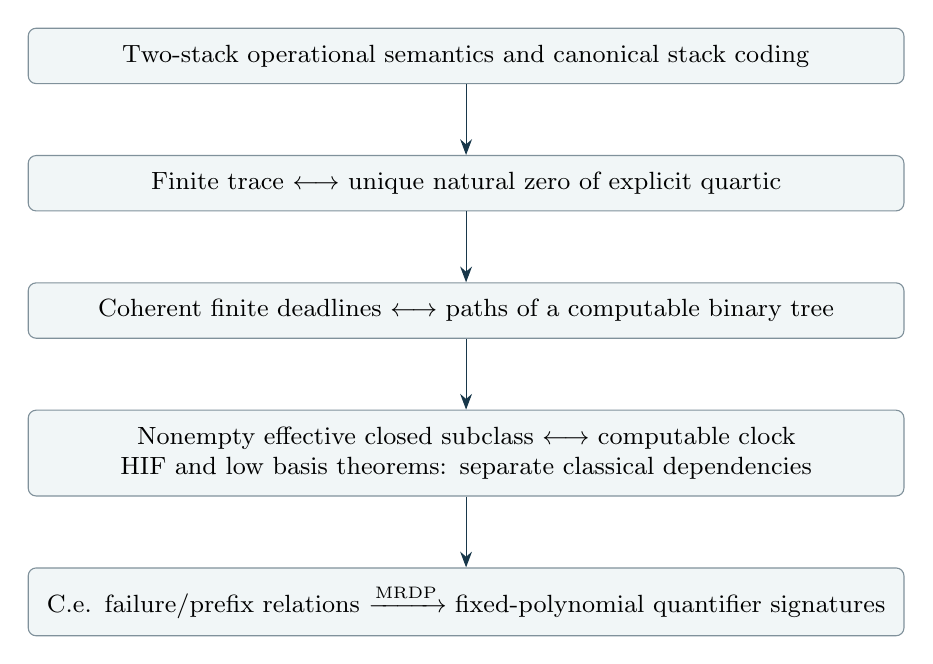
\begin{tikzpicture}[node distance=9mm,
 box/.style={draw=ink!55,rounded corners=1mm,fill=wash,
 text width=10.7cm,align=center,inner sep=6pt,font=\small},
 arr/.style={-{Stealth[length=2mm]},draw=ink}]
\node[box] (sem) {Two-stack operational semantics and canonical stack coding};
\node[box,below=of sem] (poly) {Finite trace $\longleftrightarrow$ unique natural zero of explicit quartic};
\node[box,below=of poly] (clock) {Coherent finite deadlines $\longleftrightarrow$ paths of a computable binary tree};
\node[box,below=of clock] (basis) {Nonempty effective closed subclass $\longleftrightarrow$ computable clock\par
HIF and low basis theorems: separate classical dependencies};
\node[box,below=of basis] (mrdp) {C.e. failure/prefix relations $\xrightarrow{\text{MRDP}}$
fixed-polynomial quantifier signatures};
\draw[arr] (sem)--(poly);
\draw[arr] (poly)--(clock);
\draw[arr] (clock)--(basis);
\draw[arr] (basis)--(mrdp);
\end{tikzpicture}
\end{center}

The arrows show a sensible implementation order, not that the MRDP theorem
logically needs the basis theorems. In fact, the arithmetic signatures can
be proved after the clock compactness theorem without any HIF construction.

\subsection{Suggested module boundaries}
A practical Lean development could use the following conceptual modules;
these are proposed names, not assertions that the files already exist.

\paragraph{\code{Liveness/Operational.lean}.}
Define an effective binary transition system, finite execution by recursion,
accepting counts, and the $k$th visit relation. Prove that a finite schedule
fixes every configuration and count. Keep totalized rejecting behavior
explicit rather than using an implicit convention for halted paths.

\paragraph{\code{Liveness/Deadlines.lean}.}
Define finite coherent deadline feasibility and its recursive binary tree.
Prove prefix closure and the exact path characterization. Establish
\cref{thm:compact} through a clearly identified compactness or K\"onig
lemma interface, rather than introducing an axiom named after the desired
liveness theorem.

\paragraph{\code{Liveness/TwoStackQuartic.lean}.}
Define finite rule syntax, canonical stack coding, the variable-index sum
type, and a polynomial generator. The critical theorem is an equivalence
between a labelled trace and the generated constraints, followed by
uniqueness of guard and deadline slacks. The sum-of-squares implication
should be proved over integers, and only then used for natural valuations.
The variable and residual counts become cardinality calculations on the
index types. Python can generate examples, but the mathematical compiler
must itself have a correctness proof.

\paragraph{\code{Liveness/ClockDegrees.lean}.}
Define computable domination and the deadline oracle spectrum on genuine
oracle-recursion semantics. The easy implication from an HIF accepting
schedule to a computable clock uses only the oracle computation of the
$k$th accepting time. The reverse direction should depend on a separately
formalized and audited HIF basis theorem. The c.e.-degree realization can
be formalized independently from that basis theorem: its proof uses the
explicit enumeration modulus and unary-cost bound.

\paragraph{\code{Liveness/Diophantine.lean}.}
Apply \code{Diophantine.mrdp} to the c.e. relations
$\operatorname{Bad}_d$, $\operatorname{BadGap}$, and $V^*$.
Do not try to prove these temporal properties themselves c.e.; that is
exactly what the no-go theorem excludes. Keep the compiler for a concrete
finite trace distinct from a general MRDP witness extractor.

\paragraph{\code{Liveness/AffineRealization.lean}.}
Prove rational push/pop identities and rule-by-rule preservation on the
subset of encoded finite stacks. Only afterward define the arbitrary
completion of the map on the rest of the cube. The proof need not decide
whether every real point is a valid finite stack code. The fourth-coordinate
construction additionally requires the convergent digit series and its
computable inverse on the separated Cantor set.

\subsection{Proof obligations most likely to conceal an error}
The important boundary checks are short enough to list explicitly.
\begin{enumerate}[label=\textnormal{(\arabic*)}]
\item Prefix coherence: the length-$d(k)$ certificate must include every
$j\le k$ deadline, not merely the final acceptance count.
\item Finite branching: computable reachability of arbitrary long finite
paths is not itself a substitute for a computably bounded finite successor
list when extracting the effective compact tree.
\item Oracle scope: totality of a chosen schedule program is not equivalent
to existence of an arbitrary schedule; a computable clock does not imply
that its witnessing branch is computable.
\item Slack uniqueness: all inactive top slacks must be forced to zero,
and active quotients must represent a positive sentinel tail.
\item Timing preservation: acceptance flags must have the stated microstep
semantics, especially in the bounded-gap reductions.
\item Domains and arities: natural witnesses, real state coordinates,
finite-horizon variable counts, and fixed MRDP witness dimensions must not
be conflated.
\end{enumerate}
These checks identify the actual mathematical proof boundary. Merely
successfully type-checking an abstract theorem about an incorrectly defined
``trace'' or ``scheduler'' would not establish the intended result.

\section{Further research questions and concrete next targets}\label{sec:questions}

The questions below are proposed research directions. They are not all
asserted to be previously published open problems. Each is a specific
extension or optimization left unresolved by this article, rather than
an invitation to remove a quantifier that the proved hierarchy forbids.

\begin{question}[Deadline spectra beyond c.e. cones]\label{q:spectra}
Which upward-closed classes of Turing degrees occur as
$\operatorname{Spec}_{\mathrm{clk}}(e)$ for a single input of a fixed
two-stack system? In particular, which degrees can be a least element?
\end{question}
\cref{thm:ce-spectrum} realizes every principal cone above a c.e. degree.
Its proof uses a computable increasing enumeration and a modulus whose
upper bounds decide the enumerated set. A route beyond the c.e. case is to
study recursive trees whose paths admit domination-based recovery of a
non-c.e. set. One must separately establish that a matching deadline is
computable from that set; an arbitrary limit approximation need not have
a convergence modulus computable from its limit. Nonprincipal spectra
would distinguish ``some sufficiently strong oracle'' from a unique least
clock resource.

\begin{question}[A verified effective-closed-subclass compiler]
Can a repository implementation accept a certified computable tree
$T$ with $\varnothing\ne[T]\subseteq\cB_e$ and extract the program for a
valid deadline with a proved totality theorem?
\end{question}
\cref{prop:closed-clock} supplies the algorithm: search for a tree level
where every node has the required number of accepting visits. The hard
part of a proof assistant implementation is not polynomial arithmetic;
it is packaging the compactness argument that proves termination of every
search. An initial target can avoid HIF degrees entirely and establish a
usable bridge from safety invariants to explicit progress programs.

\begin{question}[Primitive-recursive and resource-bounded clocks]
What are the sharp index classifications and degree-theoretic analogues
when deadlines are required to be primitive recursive, elementary, or
polynomially bounded in $k$?
\end{question}
A computable deadline permits arbitrarily expensive total computation.
Uniform syntactic families of total clocks change the quantifier accounting:
for an effectively listed total family $(d_m)$, the existence condition has
an immediate $\exists m\forall k$ upper bound, unlike the general
$\sig3$ condition that must verify totality. Establishing sharp lower
bounds requires simulations whose pulse costs fit that family. The HIF
basis argument by itself supplies no elementary or polynomial bound.

\begin{question}[Clock synthesis under regular reachability abstractions]
Which effective regular abstractions certify a nonempty closed subclass
of accepting schedules, and when do they compute useful deadlines?
\end{question}
To--Libkin-type recurrent reachability procedures and their recent
extensions exploit effective regularity assumptions \cite{ek2025}.
A promising bridge is to turn a regular recurrent witness into a recursive
schedule tree with a quantified progress guarantee. The key task is to
prove that an abstract infinite path corresponds to a concrete path;
a regular overapproximation may contain recurrent behavior absent from
the concrete system. The deadline extraction should be conditional on a
proved simulation or refinement relation, not just apparent recurrence in
an abstraction.

\begin{question}[Probabilistic and adversarial progress]
How do computable deadlines interact with almost-sure recurrence,
positive-probability recurrence, and strategies that work against every
adversary?
\end{question}
These quantifiers are different from existential selection of one schedule.
Recent regular-model-checking work treats both sure and almost-sure
properties under explicit hypotheses \cite{ek2025}. For the present
framework, one concrete target is a measure-theoretic substitute for the
closed-subclass condition: does a positive-measure computable-deadline
class exist whenever recurrence has a specified effective probability
bound? Another target is to formalize the precise order of strategy,
opponent, time-bound, and probability quantifiers before attempting any
Diophantine compilation.

\begin{question}[Minimal geometric dimension and regularity]
Can the clock and c.e.-degree-spectrum realizations be achieved with fewer
coordinates or stronger regularity, while retaining a finite rational
input encoding and an explicitly stated scheduler domain?
\end{question}
The construction here uses three coordinates for a controlled relation
and four for an autonomous map with a scheduler parameter. It does not
claim optimality. Reducing dimension by interleaving codes may destroy
piecewise-affineness or the finite guard partition. Requiring continuity,
invertibility, or a smooth flow creates separate obligations. Any candidate
should first establish a step-exact or computable signal-faithful simulation,
then determine which fixed deadlines or gap bounds survive.

\begin{question}[Robust encodings and noise]
What survives under bounded perturbations, finite precision, or a
noise-tolerant decoding rule?
\end{question}
The current rational codes represent unbounded information at ever finer
scales. Noise can erase low-order digits, so compact exact universality
alone says nothing about robustness. An appropriate problem is to specify
an error model and prove either a robust simulation contract or an
impossibility theorem for a chosen deadline class. This should be treated
as a change of mathematical model, not as an implementation detail of the
exact construction.

\begin{question}[Other unconventional substrates with timing certificates]
Can one build clock-faithful translations to interaction nets,
contextual rewriting, tiling-based computation, or reaction systems with
an explicit effective zero-test mechanism?
\end{question}
The useful deliverable would be a simulation theorem satisfying
\cref{thm:transfer}, plus a local polynomial compiler for the target's own
finite steps. Mere finite-halting universality is insufficient. The first
obligations are termination of administrative phases, absence of
accepting internal divergence, and effective bounds on all finite
simulation trees. Restricting to a model with no zero tests may radically
change its computational power, so the operational language must be fixed
before importing universality claims.

\begin{question}[Smaller exact local certificates]
Can the counts $H(3+R+G)+k$ and $H(4R+E+2G+2)+k$ be improved without
losing the labelled-trace bijection or raising degree above four?
\end{question}
Possible savings include eliminating deterministic rule selectors,
sharing guards when their active conditions are provably disjoint, and
using a different control encoding. Each change should include a new
witness-uniqueness proof; eliminating inactive-slack equations without
an alternative canonicalization is not a valid optimization. Lower bounds
for natural quadratic encodings of guarded affine transitions would also
be informative. The present counts are exact for this compiler, not
optimal across all compilers.

\begin{question}[Concrete fixed-arity MRDP extraction]
Can the three c.e. relations used in \cref{thm:polynomial-signatures} be
compiled to explicit fixed polynomials with audited witness counts,
operation counts, and a verified correspondence to the programs?
\end{question}
The repository's MRDP existence theorem is already enough for the logical
normal forms. A practical extractor would require a compiler for the
particular program semantics and an explicit accounting of all arithmetic
encodings. This project should not begin by promising preservation of
single-fold witnesses: \cref{rem:singlefold} marks that as a separate and
substantially stronger issue.

\begin{question}[Quantitative certificates for the degree realizations]
Can one export finite prefixes of the c.e.-degree spectrum construction
as exact quartic certificates together with a formal proof that every
successful deadline computes the intended c.e. set?
\end{question}
This is a focused near-term project combining the most concrete parts of
the article. It needs a standard bounded enumeration machine, the tree
predicate \cref{eq:c.e.-tree}, a verified unary-cost lower bound, and the
finite compiler. Finite examples alone cannot certify the lower-degree
claim, but they can exercise every arithmetic component used by its proof.

\begin{question}[The mass problem of finding a recurrent schedule]
How do the solution sets $\cB_e$, their nonempty effectively closed
subclasses, and their computable-deadline unions compare under uniform
and nonuniform reductions between mass problems?
\end{question}
\cref{thm:core} characterizes nonemptiness of the computably clocked part
through HIF solutions, but it does not provide a uniform algorithm selecting
a schedule from a clock. The DNR example rules out the most naive selector.
A finer classification could separate the difficulty of finding a clock,
finding a closed subclass, and selecting a path inside that subclass.
This is especially relevant to proof-producing synthesis systems, where
``there exists a strategy'' and ``a strategy can be extracted uniformly''
are operationally very different outputs.

\section{Conclusion}

The decisive boundary in Diophantine compilation is not the aesthetic form
of the computational substrate. It is the information content and
quantifier structure of the requested behavior. Finite successful
computations are c.e. and hence Diophantine. Recurrent behavior requires
coherent infinite choices, and finite branching alone does not remove that
requirement.

A shared computable progress deadline supplies precisely the compactness
needed to pass from coherent finite certificates to an infinite execution.
It is equivalent to a nonempty effectively closed family of accepting
schedules and, through the classical basis theorem, to the existence of an
HIF accepting schedule. The degree-spectrum construction gives a separate
quantitative answer: every c.e. degree can be exactly the minimum oracle
strength needed to compute a successful clock. The halting-degree instance
has accepting runs but no computable deadline at all.

These results coexist with a completely explicit finite arithmetization.
The two-stack compiler uses natural witnesses and quadratic residuals,
producing a nonnegative quartic with a proved labelled-trace bijection.
The same computations occur in a compact rational guarded affine system;
adding a real scheduler coordinate turns it into a deterministic map while
making the initial-parameter quantifier visible. Fixed-arity MRDP then
provides the correct alternating polynomial signatures, rather than an
invalid universal existential representation of liveness.

The immediate research value is a precise architecture for extending
ProveIt: exact finite compilers, coherent deadline trees, separately audited
basis and degree arguments, and explicit arithmetic quantifier boundaries.
This architecture makes both positive representations and impossibility
results testable against the intended operational semantics.

\appendix
\section{Reproduction and artifact manifest}\label{app:reproduction}

From the archive root, run:
\begin{lstlisting}[language=bash]
python3 code/test_clock_compiler.py
python3 code/clock_compiler.py
latexmk -pdf -interaction=nonstopmode -halt-on-error beyond_halting.tex
\end{lstlisting}
The Python programs use the standard library only. The LaTeX source uses
standard TeX Live packages, including New PX fonts, AMS mathematics,
Microtype, TikZ, and \code{tcolorbox}. Alternatively, run pdfLaTeX three
times to resolve the table of contents and cross-references. No external
bibliography processor is required.

\begin{center}
\begin{tabular}{@{}p{0.48\linewidth}p{0.45\linewidth}@{}}
\toprule
File & Purpose\\
\midrule
\code{beyond\_halting.tex} & Complete editable article source.\\
\code{beyond\_halting.pdf} & Rendered and visually checked article.\\
\code{code/clock\_compiler.py} & Exact finite-horizon polynomial compiler and sample export.\\
\code{code/test\_clock\_compiler.py} & Reproducible finite arithmetic tests.\\
\code{artifacts/example\_certificate.json} & Full 52-variable, 137-residual sample and witness.\\
\code{artifacts/test\_report.json} & Results from the executed tests.\\
\code{README.md} & Build commands, scope, and proof-status summary.\\
\code{research/source\_ledger.md} & Inspected source references and provenance boundaries.\\
\bottomrule
\end{tabular}
\end{center}

\clearpage
\section{A compact theorem-dependency ledger}\label{app:dependencies}
\begin{longtable}{@{}p{0.27\linewidth}p{0.38\linewidth}p{0.27\linewidth}@{}}
\toprule
Endpoint & Principal ingredients & Verification status\\
\midrule
\endfirsthead
\toprule
Endpoint & Principal ingredients & Verification status\\
\midrule
\endhead
Coherent compactification & Finite run semantics; computable binary tree; K\"onig compactness & Conventional proof.\\
Clock/closed/HIF equivalence & Compactification; uniform bounds on a compact class; classical HIF basis & Conventional proof; basis attributed.\\
C.e.-degree spectrum & Bounded enumeration tree; unary cost; enumeration modulus & Conventional explicit construction.\\
Hierarchy upper bounds & Finite decidability; common program index; analytic schedule quantifier & Conventional proof.\\
Hierarchy lower bounds & Unary witness selection; decidable search; recursive-tree normal form & Conventional reductions; recurrence endpoint classical.\\
Finite quartic bijection & One-hot indicators; canonical sentinel stacks; inactive slack equations & Conventional proof and finite exact tests.\\
Compact affine realization & Rational push/pop identities; finite linear guards & Conventional proof and exact identity tests.\\
Initial-parameter hierarchy & Cantor digit coding; rational periodicity; schedule-degree equivalence & Conventional proof.\\
Fixed-polynomial forms & MRDP; polynomial parameter pairing; quadratic circuit lifting & Classical backend; no general extractor implemented.\\
No-go theorem & Diophantine sets are c.e.; strict hierarchy and analytic hardness & Conventional consequence.\\
\bottomrule
\end{longtable}

\clearpage
\begin{thebibliography}{99}
\small\raggedright

\bibitem{proveit-mrdp}
Vladimir Reshetnikov, \emph{ProveIt: Diophantine/MRDP.lean},
repository source at commit
\code{b6bf6406a4c49017fedc6fba068b36c634987150}, inspected September 30, 2026.
\href{https://github.com/VladimirReshetnikov/ProveIt/blob/b6bf6406a4c49017fedc6fba068b36c634987150/Computability/HilbertTenthProblem/Lean/Diophantine/MRDP.lean}{Pinned theorem source}.

\bibitem{proveit-guide}
Vladimir Reshetnikov, \emph{MRDP: recursively enumerable if and only if
Diophantine}, ProveIt repository guide, revision
\code{b998f70c6886e6a00339a6f4a02ed8625324d357}, inspected September 30, 2026.
\href{https://github.com/VladimirReshetnikov/ProveIt/blob/b998f70c6886e6a00339a6f4a02ed8625324d357/Computability/HilbertTenthProblem/Lean/MRDP.md}{Pinned MRDP guide}.

\bibitem{proveit-degrees}
Vladimir Reshetnikov, \emph{Turing degrees in Lean and Rocq},
ProveIt repository README, revision
\code{b998f70c6886e6a00339a6f4a02ed8625324d357}, inspected September 30, 2026.
\href{https://github.com/VladimirReshetnikov/ProveIt/blob/b998f70c6886e6a00339a6f4a02ed8625324d357/Computability/TuringDegrees/README.md}{Pinned Turing-degree project guide}.

\bibitem{matiyasevich1970}
Yuri V. Matiyasevich, ``Enumerable sets are Diophantine,''
\emph{Soviet Mathematics Doklady} \textbf{11} (1970), 354--358.
English translation of \emph{Doklady Akademii Nauk SSSR} \textbf{191}
(1970), 279--282. Reprinted in \emph{Mathematical Logic in the 20th Century}
(2003), DOI: \href{https://doi.org/10.1142/9789812564894_0013}{10.1142/9789812564894\_0013}.

\bibitem{js1972}
Carl G. Jockusch, Jr. and Robert I. Soare,
``$\Pi^0_1$ classes and degrees of theories,''
\emph{Transactions of the American Mathematical Society} \textbf{173}
(1972), 33--56.
DOI: \href{https://doi.org/10.1090/S0002-9947-1972-0316227-0}{10.1090/S0002-9947-1972-0316227-0}.

\bibitem{ng2013}
Keng Meng Ng, Frank Stephan, Yue Yang, and Liang Yu,
``Computational aspects of the hyperimmune-free degrees,''
in \emph{Proceedings of the 12th Asian Logic Conference},
World Scientific, 2013, 271--284.
DOI: \href{https://doi.org/10.1142/9789814449274_0015}{10.1142/9789814449274\_0015}.
Author manuscript: \url{https://personal.ntu.edu.sg/kmng/Files/Papers/hif_ALC.pdf}.

\bibitem{hps}
David Harel, Amir Pnueli, and Jonathan Stavi,
``Propositional dynamic logic of nonregular programs,''
\emph{Journal of Computer and System Sciences} \textbf{26}(2)
(1983), 222--243.
DOI: \href{https://doi.org/10.1016/0022-0000(83)90014-4}{10.1016/0022-0000(83)90014-4}.
The recurrent-machine completeness endpoint is Proposition 5.1,
also explicitly cited and stated in \cite{ek2025}.

\bibitem{cf2011}
Krishnendu Chatterjee and Nathana\"el Fijalkow,
``Finitary languages,'' 2011.
\url{https://arxiv.org/abs/1101.1727}.

\bibitem{moore1990}
Cristopher Moore, ``Unpredictability and undecidability in dynamical systems,''
\emph{Physical Review Letters} \textbf{64} (1990), 2354--2357.
DOI: \href{https://doi.org/10.1103/PhysRevLett.64.2354}{10.1103/PhysRevLett.64.2354}.
Author summary: \url{https://sites.santafe.edu/~moore/pubs/gs.html}.

\bibitem{ek2025}
Javier Esparza and Valentin Krasotin,
``Regular model checking for systems with effectively regular reachability
relation,'' in \emph{50th International Symposium on Mathematical
Foundations of Computer Science (MFCS 2025)},
\emph{Leibniz International Proceedings in Informatics} \textbf{345},
article 45, 2025.
DOI: \href{https://doi.org/10.4230/LIPIcs.MFCS.2025.45}{10.4230/LIPIcs.MFCS.2025.45}.
Full version: \url{https://arxiv.org/abs/2506.18833}.

\end{thebibliography}
\end{document}
